%% ----------------------------------------------------------------
%% Thesis.tex -- MAIN FILE (the one that you compile with LaTeX)
%% ---------------------------------------------------------------- 

% Set up the document
\documentclass[a4paper, 11pt, oneside]{Thesis}  % Use the "Thesis" style, based on the ECS Thesis style by Steve Gunn

% Include any extra LaTeX packages required
\usepackage[square, numbers, comma, sort&compress]{natbib}  % Use the "Natbib" style for the references in the Bibliography
\usepackage[nottoc]{tocbibind} % bind bibliography to the table of contents
\usepackage{verbatim}  % Needed for the "comment" environment to make LaTeX comments
\usepackage{vector}  % Allows "\bvec{}" and "\buvec{}" for "blackboard" style bold vectors in maths
\usepackage[table]{xcolor}
\hypersetup{urlcolor=black, colorlinks=true}  % Colours hyperlinks in black, can be distracting if there are many links and colored blue.
\usepackage{graphicx}
\graphicspath{{Figures/}}  % Location of the graphics files (set up for graphics to be in PDF format)

%% ----------------------------------------------------------------
\begin{document}
\frontmatter      % Begin Roman style (i, ii, iii, iv...) page numbering



% Set up the Title Page
\title  {\thesistitle}
\authors{\studentname}
            
\addresses  {\groupname\\\deptname\\\univname}  % Do not change this here, instead these must be set in the "Thesis.cls" file, please look through it instead
\date       {\today}
\subject    {}
\keywords   {}

\maketitle
%% ----------------------------------------------------------------

\setstretch{1.3}  % It is better to have smaller font and larger line spacing than the other way round

% Define the page headers using the FancyHdr package and set up for one-sided printing
\fancyhead{}  % Clears all page headers and footers
\rhead{\thepage}  % Sets the right side header to show the page number
\lhead{}  % Clears the left side page header

\pagestyle{fancy}  % Finally, use the "fancy" page style to implement the FancyHdr headers

%% ----------------------------------------------------------------
% Declaration Page required for the Thesis
\Declaration{

\addtocontents{toc}{\vspace{1em}}  % Add a gap in the Contents, for aesthetics


      
This report, \thesistitle, is submitted in partial fulfillment of the requirements of \awardlevel \space in \award \space at \institutename. I, \studentname , declare that this thesis titled, \thesistitle and the work represents substantially the result of my own work except where explicitly indicated in the text. This report may be freely copied and distributed provided the source is explicitly acknowledged. I confirm that:

\begin{itemize} 
\item[\tiny{$\blacksquare$}] This work was done wholly or mainly while in candidature \awardlevel \space in \award \space at \institutename.
 
\item[\tiny{$\blacksquare$}] Where any part of this thesis has previously been submitted for a degree or any other qualification at \institutename \space or any other institution, this has been clearly stated.
 
\item[\tiny{$\blacksquare$}] Where I have consulted the published work of others, this is always clearly attributed.
 
\item[\tiny{$\blacksquare$}] Where I have quoted from the work of others, the source is always given. With the exception of such quotations, this project report is entirely my own work.
 
\item[\tiny{$\blacksquare$}] I have acknowledged all main sources of help.
 
\item[\tiny{$\blacksquare$}] Where the thesis is based on work done by myself jointly with others, I have made clear exactly what was done by others and what I have contributed myself.
\\
\end{itemize}
 
 
Signed:\\
\rule[1em]{25em}{0.5pt}  % This prints a line for the signature
 
Date:\\
\rule[1em]{25em}{0.5pt}  % This prints a line to write the date
}
\clearpage  % Declaration ended, now start a new page

%% ----------------------------------------------------------------

% The Abstract Page
\addtotoc{Abstract}  % Add the "Abstract" page entry to the Contents
\abstract{
\addtocontents{toc}{\vspace{1em}}  % Add a gap in the Contents, for aesthetics
Autism spectrum disorders are a group of complex neurodevelopmental conditions that affected individuals social interactions, communication, and repetitive and stereotyped behaviours and patterns. Computer-based instructions and technology in the classroom may affect the development of social skills among students, especially those on the autism spectrum and potentially help with their education and learning phases. There are various types of technology used in the classroom including gamification, assistive technologies, interfaces, portable devices, robotic devices, software, and videos. At the same time, focusing on instructional technology and assistive technology and how they can positively impact children with Autism and their education. Technology can allow computer-based instructions to be repeated; this can benefit an Autism Child who has repetitive behaviours and patterns; meaning the Children are not overwhelmed as they can engage and interact at their own pace and level of learning. Research has been carried out in diagnosing and early intervention of a child with Autism; there is a lack of research in the formal education of Autistic Children and technology. As technology use, design, devices and target markets, meaning gaps in technology for Autistic children. The untapped potential in everyday potential technological devices as educational aids and tools could be huge for children with Autism.

Line of how i am different
}

\clearpage  % Abstract ended, start a new page
%% ----------------------------------------------------------------

\setstretch{1.3}  % Reset the line-spacing to 1.3 for body text (if it has changed)

% The Acknowledgements page, for thanking everyone
\acknowledgements{
\addtocontents{toc}{\vspace{1em}}  % Add a gap in the Contents, for aesthetics
The acknowledgements and the people to thank go here, don't forget to include your project supervisor\ldots

}
\clearpage  % End of the Acknowledgements
%% ----------------------------------------------------------------

\pagestyle{fancy}  %The page style headers have been "empty" all this time, now use the "fancy" headers as defined before to bring them back


%% ----------------------------------------------------------------
\lhead{\emph{Contents}}  % Set the left side page header to "Contents"
\tableofcontents  % Write out the Table of Contents

%% ----------------------------------------------------------------
\lhead{\emph{List of Figures}}  % Set the left side page header to "List if Figures"
\listoffigures  % Write out the List of Figures

%% ----------------------------------------------------------------
\lhead{\emph{List of Tables}}  % Set the left side page header to "List of Tables"
\listoftables  % Write out the List of Tables

%% ----------------------------------------------------------------
\setstretch{1}  % Set the line spacing to 1.5, this makes the following tables easier to read
\lhead{\emph{Abbreviations}}  % Set the left side page header to "Abbreviations"
 % Include a list of Abbreviations (a table of two columns)


% \textbf{Acronym} & \textbf{W}hat (it) \textbf{S}tands \textbf{F}or \\
%\listofsymbols
%\section{Abbreviations}
%\begin{table}
	%\centering
	%	\begin{tabular}{ c c }\toprule[1.5pt]
	%	\hline
	%	AI & Artificial Intelligence  \\
	%	AR & Augmented Reality \\
	%	ASC & Autism Spectrum Conditions \\
	%	ASD & Autism Spectrum Disorder \\
	%	CNN & Convolutional Neural Network \\
	%	DL & Deep Learning \\
	%	ICT & Information and Communication Technology \\
	%	IEP & Individualised Education Plans \\
	%	IL & Interactive Learning \\
	%	RNN & Recurrent Neural Network \\
	%	SNAs & Special Needs Assistants \\
	%	\end{tabular}
%	\label{tab:Mylar}
%\end{table}


%% ----------------------------------------------------------------
% End of the pre-able, contents and lists of things
% Begin the Dedication page

\setstretch{1.3}  % Return the line spacing back to 1.3

\pagestyle{empty}  % Page style needs to be empty for this page
\dedicatory{For/Dedicated to/To my\ldots}

\addtocontents{toc}{\vspace{2em}}  % Add a gap in the Contents, for aesthetics

%% ----------------------------------------------------------------
\mainmatter	  % Begin normal, numeric (1,2,3...) page numbering
\pagestyle{fancy}  % Return the page headers back to the "fancy" style

%% ----------------------------------------------------------------
%% CHAPTERS
\chapter{Introduction}
\label{chap:intro}
\lhead{\emph{Introduction}}


The topic of this thesis is understanding how augmented reality and artificial intelligence can impact the education of an individual with Autism through conducting surveys, interviews and a proposed prototype design for testing. This thesis will describe in detail the current availability of computer-based instruction applications for individuals with Autism, through researching existing materials available online. There will be a comparison table of how it affected the individuals learning, if the outcome had a negative or positive impact or if the results were inconclusive. Autism Spectrum Disorders are a complex group of neurodevelopmental disabilities; in the 2016 Irish census, it has been recorded that 66,611 people or 1.4 per cent of the population, suffered from an intellectual disability, 8,902 higher than in 2011, showing a 15.4 per cent increase. The previous census information showed 10 to 14-year-old males, with 5,233 affected in this age group - more than double females (2,284)~\cite{Reference1}, the relevance to this information is that there is a rise in individuals being diagnosed with Autism and predominately in males. Studies demonstrate the difference in the estimated rates of Autism between the genders, males are more likely to be diagnosed with Autism than females. There is existing evidence to suggest that ASD prevalence rates, and needs for services, are higher in disadvantaged areas~\cite{Reference2}. This thesis will discuss a proposed prototype design based on the feedback from the surveys conducted; it is developed with trained professionals and based on school books to ensure it follows the current educational system. The study will include a table of the hypothesis for comparison and how the participants reacted to the short demos. This niche area focuses on a minority of the Irish population, it focuses again on the school-goers of the minority. The scope for this study is and research is extensive due to the ever-changing diagnosis of ASD, their change in needs and behaviours and the influence that technology can have on individuals. The studies are predominately recent as technology became more accessible and affordable globally, the rates of individuals in Ireland with ASD as seen in the 2016 census. The United States have seen an increase in Autism since 2001; the awareness of Autism is raised due to the rise in diagnosis~\cite{Reference3}. The increase in further research in Autism is because of the rise in diagnosis, meaning an increase of individuals with ASD within society with their ever-changing needs that modern society will have to adapt to and develop learning strategies for both students and teachers for the best outcome in the education of individuals with Autism. The current situation and resources based on AR, VR and AI are available to children with ASD. However, traditional teaching methods, such as books, are still the standard form of strategies used in a schooling environment. This thesis hypothesises that children with ASD respond better to computer-based instruction applications due to their social and motor limitations, asking why there is not a higher prevalence of computer-based instruction applications being used in the education of students with ASD. The increase in diagnosis and the increase of those being school-goers are possibly having their educational needs neglected due to the system for students who are developing typically, or typical is being used instead of an individual, child-centred approach being used in the classroom. The resources available in the class, the ratio of students to the teacher must be assessed and considered for future studies. The limitation of resources impacts the results. Children with Autism are considered to be visual learners. Hence, many scientifically proven audio-visual teaching approaches like Picture Exchange Communication Systems (PECS) and visual routines are incorporated into the education of Children and ASD~\cite{Reference4} Children with ASD typically respond better to computer-based instructions, RNN and CNN. Teaching children with special needs is a personalised activity that includes creating planned Individualised Education Plans (IEPs). These IEPs cover all the aspects of day-to-day life activities and tasks, from education to social interaction to personal hygiene. Along with planning and preparing IEPs, teaching includes creating lesson plans and lesson content and making logs for progress tracking. Implementing assisting aids to automate the activities mentioned above using Information and Communication Technology (ICT) will make processes more manageable and consistent. Mobile-based Augmented Reality (AR) is a multimedia-based technology that can cause computer objects to interact and engage with the Child using any handheld smart device. Augmented Reality (AR) enhances or augments reality by overlaying it with useful computer-generated graphics or virtual objects. AR applications can be of two types: marker-based or markerless AR. Markers are the optical inputs that an AR application recognises and tracks in a video stream.
AR can serve as an effective technology in developing a teaching/learning tool in real-time and increase motor skills, cognitive skills and overall increase brain development. AR can be used to track hand movement, eye movement, and behaviours~\cite{Reference5}.
% needs to be approx 1000 words
% Putting in comments within the TeX file can help make notes for yourself and dump text that you intend to edit later

\section{Motivation}
The education of Children with Autism is essential to me. I have a family member on the spectrum. I saw how his delayed development impacted his learning from a young age. Traditional education practices are not personalised towards children, especially those with learning disabilities. I have developed multiple projects for Children with special needs. As a spokesperson for people with disabilities, I decided to create a project that will positively impact children with ASD and their education.

\section{Ethical issues in the research}

\section{Research Objectives}
My research objectives are;
\begin{enumerate}
    \item To explore and research the impact AR and AI have on the Education of Autistic Children through interviews, surveys and proposed prototype design testing.
    \item Carry out primary research on the impact of computer-based instructions on Children with Autism.
\end{enumerate}

\section{Contribution}
The contribution of this research paper introduces the novelty of introducing AR and AI computer-assisted learning for Children specifically with ASD. This paper will research the use of AR and AI with no addition of physical books or QR codes. This research differs from existing information as educational professionals will be interviewed and other professionals in the field, such as SNAs and Special Needs Teachers. Surveys will be conducted with a broader range of design professionals, e-Learning designers and developers on the design and how it can be implemented into a class of Children with Autism. 

%Specify the problem. List your project goals and research questions here. Enumerate the main contributions. How have you advanced state of the art, i.e. what have you done that is new?

\section{Structure of This Document}
% notice how I cross-referenced the chapters through using the \label tag --> LaTeX is VERY similar to HTML and other markup languages, so you should see nothing new here!
%Introduce the structure of your report. This section is quite formulaic. Briefly describe this document's design, enumerating what each chapter and section stands for. For instance, in this work in Chapter \ref{chap:litreview} the guidance in structuring the literature review is given. Chapter \ref{chap:design} describes the main requirements for the problem definition and so on ...

\section{Research Methodology}

Respondents for the surveys are selected to ensure that the quality of responses is to a high standard; they are chosen based on their expertise, either in disability diagnostics, education for mainstream children and education for individuals with Autism, parents for Children with disabilities. However, the target audience for the AR testing is smaller. The feedback from surveys is on quality responses rather than on the number of responses. Further information on the data collection method is provided in the Research Methodology chapter.

\section{Prototype}

Following research on augmented reality and artificial intelligence applications and how they impacts an Autistic child's education. A prototype will be designed and based roughly on previous learning applications, the prototype was designed to simulate how AR would be presented in a classroom and how it can be used to educate children with Autism through a child-centred strategy, the Child would go at their pace, and it would be individualised lessons. Excessive amounts of research has been completed on the workings of augmented reality, including the complex technology involved and possible future developments. The research methodology chapter identifies how the data is collected for the research and why this particular method was chosen. The prototype and design testing chapter explains the path taken to develop the prototype from concept to the final version. The results and analysis chapter examines the responses from the four surveys and seven interviews. These findings are then analysed in the Results and Analysis chapter. Further discussion on the methodology chosen is then given in the Discussion chapter. To conclude at the end of the thesis, a conclusion provides some final thoughts on the research and further work and development. 


 % Introduction
\chapter{Research background}
\label{chap:Research background}
\lhead{\emph{Research background}}

\section{What is Autism?} 

To understand how an individual with Autism functions and reacts to computer-based instructions, it has to describe what Autism is and how their learning and social skills are affected. Autism is a developmental delay and disability that affects social interaction, social communication and social imagination; this is known as the triad of impairments~\cite{Reference6}. 

The first of the triad is social interaction; the person with Autism may not have an interest in a particular activity. It can be challenging for them to make friends with other individuals and individuals their age and typically have difficulties with maintaining eye contact; it may either be absent or indifferent. When a person with Autism does not initiate conversation or find it challenging to continue a conversation, they may also experience delayed language development and usually have a repetitive language or behaviour; this is the social communication impairment of the triad. The last of the triad is social imagination; individuals with Autism may not imagine what will happen, they often lack hindsight. Next, they may have limited creative skills or imaginative play; this affects their ability to keep or access information or memories related to personal experiences~\cite{Reference7}.

The triad of impairment in each person with ASD can differ based on the severity of the disability, individuals level of intelligence, personality traits, the presence of other disorders and if there has been the introduction of additional resources to improve the individuals disorder. Individuals with ASD may also experience sensory issues and be hypersensitive to smell, sound, taste, touch and visual stimulation. The world of a person with ASD can be challenging and confusing, to both the individual with Autism and those who are typically functioning. Individuals with ASD may rely on repetitive patterns and behaviours, become attached to particular physical objects, and only consume specific foods and drinks. People with ASD may lack responsiveness due to the triad of impairments, this is sometimes mistaken for being deaf or struggling with hearing ~\cite{Reference8}.

\section{Autism in education} 

In 2016, it was seen that 1 in 65 of the school-going population has a diagnosis of Autism~\cite{Reference9}.
It has been proven from existing research that children with Autism benefit greatly from education that is especially suited to their needs by educational professionals. The approaches must be widely available and ethical, so it does not cause distress to the person with Autism~\cite{Reference10}. The National Council for Special Education in Ireland details practical teaching strategies for students with Autism. Children with ASD can benefit from a combination of custom teach strategies, also known as an eclectic approach. This is when two or more strategies are combined for the student and their individual needs, this is a child-centred approach, this personalised approach is recommended for children with learning disabilities. Strategies listed include Lámh (language alternative for the mentally disabled), a manual signing language designed for individuals with ASD and other learning disabilities in Ireland. Another strategy that focuses on the individual teaching strategies for children with learning disabilities discussed is Teacch, originating from North Carolina and now adopted in Ireland, Teacch is a structured teaching approach for students with ASD~\cite{Reference11}. 

\section{What is Augmented Reality?}

Augmented Reality (AR) is described as the process of combining both real and computer generated assets that enhances the user's senses in vision, touch, hearing, taste and smell~\cite{Reference12}. It is described as an experience where parts of a user's physical world is combined through an immersive experience with computer-generated inputs; AR responds in real-time in the user's environment~\cite{Reference13}. AR can be dated back to 1901 and can be seen in science fiction movies; however, in 1990, Tomas Caudell described AR as a technology and how it was used to design Boeing's intricate aircraft system so workers could visualise the setup and therefore lowering human errors~\cite{Reference14}. 
% new line
 AR is under extended reality (XR) alongside virtual reality and mixed reality; AR differs from enhancing real-world views, not isolating the user from their environment, like virtual reality. Digital assets are superimposed, usually on a handheld smart device, to enhance the user's real-world environment. Pokemon Go, the mobile application released by the software company Niantic in July 2016, is an excellent real-life example of how AR works in real-time and in its environment; it uses GPS technology that inserts digital assets, the Pokemon characters, into the user's environment through a mobile device.
% new line 
 AR takes both real-world and a computer-generated world and is about how the two worlds interact with the both the real world and the digital world, it has a flexible immersion level, and the interface can be described as an out of screen experience for the users [X]. AR needs inputs and outputs; inputs from the user take form in movements, voice, controls and touch. These need to be high fidelity inputs to engage in an immersive experience. High fidelity inputs are accurate, precise and need to be comfortable for the user, while low fidelity inputs have errors, difficulties and are less precise and makes tasks increasingly difficult for the users~\cite{Reference15}.
 
 \section{How does Augmented Reality Work?}

AR incorporates computer-generated objects into a real-time environment for the user. To work it needs the following: 

\begin{itemize}
  \item Depth-sensing camera: Visual information must be recorded so computer-generated digital assets can be added to the application.
  \item Registration tools: Motion sensors and accelerometers are needed to define the space for superimposition of the digital assets into the real-world environment.
  \item Computer vision: A machine learning (ML) algorithm interprets the user's real-time environment and uses it as a reference point for the assets and their positioning. The pixels are used to recall similar-looking objects to give a high fidelity, precise and immersive experience. 
  \item Output device: This is the display where the user can experience the result; these displays can be devices such as smartphones and tablets that are widely accessible and affordable.
\end{itemize}

 \section{What are different types of Augmented Reality?}

AR enhances the user’s reality and can be carried out in different ways. 
A widely popular type of AR is Marker Based AR due to its availability and affordability. This type of AR needs an image or assets that acts as a marker for the AR technology making it more accurate and a better and more enjoyable experience for the user due to its immersive and high fidelity nature. 
\begin{itemize}
  \item Marker Based AR: This type of AR needs a distinct image or asset that acts as a marker for the technology. This type of AR is widely popular due to its availability and affordability. 
  \item Markerless AR: No marker is needed for this type of AR; you move the digital assets; an example is the international furniture company IKEA’s home remodelling application. This technology has no anchor needed for the real world.
  \item Projector based AR: This type of AR is complex and uses advanced technology. This type of technology is used in warehouses to simplify packing processes and training operations.
\end{itemize}

Augmented reality is widely used in businesses and industries to operate at their full potential and highest standard. It can be seen in industries from public safety to gaming, education, travel and equipment maintenance in both the medical and agricultural field.  

\Section {What is Artificial Intelligence?}

The definition of Artificial Intelligence is to enable computers and machines to interpret the perception, learning, problem-solving, and decision-making ability of, or as close to the human mind~\cite{Reference16}. AI is widely seen in everyday life; it can be challenging to understand due to the multiple terms, variations and interchangeable terms. AI can be linked with machine learning (ML), and deep learning (DL), speech recognition, natural language processing and can fall into either two categories of weak AI or strong AI~\cite{Reference17}.

 \section {What is difference between Artificial Intelligence, Deep Learning and Machine Learning?}
 
 \begin{itemize}
  \item Artificial Intelligence: Is the entirety of computing technology that resembles anything related to human intelligence.
  \item Machine Learning: This is a subset of AI that can learn by itself; the more data repeated to the technology helps it learn, recall and program itself for increased accuracy.
  \item Deep Learning: The models are based on deep neural networks with various layers; each layer refines the previous layer. The output layers are known as forwarding propagation and backpropagation that identify errors in calculations, and to  train the model for continuous accuracy.
\end{itemize}

 \section{What are different types of Augmented Reality?}
 
 AI can be broken into two different types, weak AI and strong AI~\cite{Reference18}.
 
  \begin{itemize}
  \item Weak AI: Described as Narrow AI or Artificial Narrow Intelligence (ANI), ANI is trained for specific tasks. Weak AI can be seen in most AI that exists. Narrow operates Apple's Siri and Amazon's Alexa.
  \item Strong AI: Artificial General Intelligence (AGI) replicates the autonomy of the human brain. AGI can choose the problems to solve without human intervention. 
\end{itemize}

AI applications and technology can be seen in everyday life; s common examples include speech to text, speech recognition, chat-bots in NPL, image recognition (computer vision or machine vision), automated stock trading and autopilot technology is only several applications using artificial intelligence functionality. 

As technology is ever evolving and changing meaning gaps in the market of technology and Autistic children are more apparent, there are numerous methods of technology such as machine learning, augmented reality, artificial intelligence, virtual reality, deep learning, gamification, convolution neural networks, and recurrent neural works have all been methods applied in the early diagnosis and intervention of a Child with ASD.Multiple research studies have been carried out in diagnosing and early intervention. However, there is a lack of research on the impact of augmented reality and artificial intelligence in the formal education of Autistic Children. This gap is significant because it gives scope for further research and development. The untapped potential in everyday technological devices as helpful tools could be huge for children with ASD. There are technological devices designed to function as tools in diagnosing and treating neurological disabilities. But, tiny amounts of technology for Autistic children and children with other developmental delays and learning disabilities and individualised technology for their additional needs.

\section{Facial expression and real time emotion computing}

Gamification plays a leading role when it comes to interaction among individuals with Autism and keeping them engaged and interactive, Paper one~\cite{Reference19} helps individuals with ASD understand other's emotions through computer-based instruction, gamification, real-time emotion computing and convolution neural networks (CNN). EmoTrain, the design concept and game engine, creates tasks that the user is expected to perform. Facial expressions and facial behaviour response skills of individuals with ASD are evaluated on the EmoTrain platform. This paper aims to improve individuals with ASD and their emotional intelligence and recognition through computer-based instructions and gamification. The papers main objectives are;

\begin{itemize}
    \item Using CNN to track facial expressions and emotions.
    \item Design EmoTrain, a real time emotion computing application to improve individuals with ASD emotional response.
    \item Understanding emotions in people 
    \texttt and improving an individual with 
    ASD and their response.
\end{itemize}

  \begin{figure}[h]
\centering
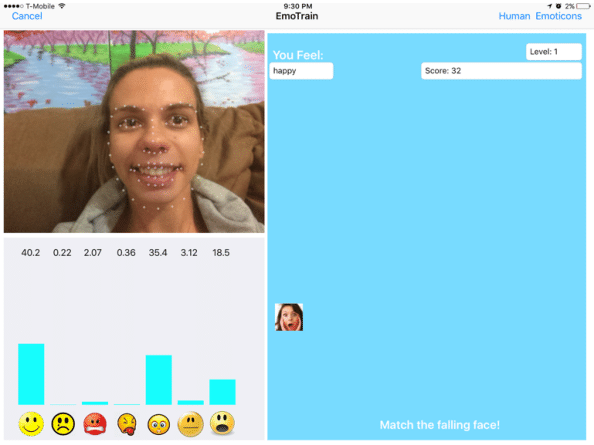
\includegraphics[width=0.5\textwidth]{IDD_LauraMartin_R00124705/Figures/emotrain.png}
\caption{EmoTrain prototype design}
\end{figure}

These objectives were tested by surveying after an evaluation study was carried out and nine subjects, aged 18 - 25 and diagnosed with ASD. Each participant received training with the EmoTrain platform two times a week, for two weeks and 20 minutes each session. 

\section{Augmented reality to improve elicit pretend play}
Children with Autism can lack in the ability to play with peers due to social and imaginative limitations, paper two~\cite{Reference20} helps children with Autism and who suffer from developmental delays with their symbolic thinking. The use of augmented reality (AR) is tested to improve elicit pretend play for Children with Autism. Areas that were focused on for improvement included individual differences, skill transfer, system usability and limitations of the proposed AR application was investigated for this paper. The design of an application for children with additional needs needs to be easy to navigate through that is why design guidelines for future AR systems for Children with ASD were also discussed for this paper. 

  This study aims to improve pretend play in children with ASC aged 4 - 7 through an interactive study that explores the possible potential of augmented reality (AR) technology taking into consideration the frequency, the duration and the relevance using the AR systems in comparison to non-computer assisted situations. 
  
  The main objectives of this paper are:
\begin{itemize}
    \item Improve pretend  play in children with Autism aged between 4 - 7 with AR implementation.  
    \item To investigate the individual differences, skill transfer, system usability, and proposed AR limitations.
\end{itemize}
  
  A  survey was conducted for both parents and the participants to collect qualitative data. The researchers considered the parents to supply more reliable data; each parent was asked to observe the participant playing and rate their engagement in cooperation, attentiveness and emotional response. Parents were also asked to complete a questionnaire; main questions included;
 
\begin{itemize}
    \item Which session do you think the participant enjoyed most?  
    \item One thing you like about the play?
    \item Are there other things you want to be on the screen?
    \item Which play is more fun?(with a friend/with the screen) and why?
\end{itemize}

Not all participants data was used for the analysis due to some participants being overwhelmed, and accurate data could not be collected. The mean frequency of pretend play recorded is higher in AR environments. Results included the mean frequency of constructive play was lower in non - AR conditions, the level of relational play, simple play and no play stays similar in both conditions, play duration was increased in AR conditions, engagement and cooperativeness are between average and high in both conditions.

\section{Autism and visual routines for effective teaching}
Children with Autism typically have visual routines introduced into their everyday life to improve social interactions and basic comprehensive understanding of everyday tasks, these visual routines act as instructions for the individual. In paper three~\cite{Reference21}  produces effective teaching, learning, and assisting aids for children with Autism and mild mental delays. The parent's voice is added to narrate the virtual 3D renderings that enhance the learning process, this comforts the child and gives them a sense of familiarity. The researchers used a mobile application that personalised AR lessons. The application supports functional reading, visual schedulers and speaking albums to learn in real-time environments.

This paper aims to implement assisting aids to automate functional reading, visual routines and picture exchange communications systems (PECS). These activities require hard copy materials. Information and communication technology (ICT) is used to make tedious activities more manageable and streamlined for parents/educators. The objectives and aims of this paper are:

\begin{itemize}
    \item To develop an e-Learning application called e-Sandhya is an accessible application for Children with ASD.  
    \item Streamline and automate functional reading, visual routines and PECS.
\end{itemize}

This paper had limitations in being validated as it failed to carry out a survey or collect any means of information for testing and validation.

\section {Autism through neuroimages and MRI data sets}

As there is increasing research into early diagnosis and intervention for an individual with Autism through neuroimages and MRI data sets. As an example of this work and research, paper four~\cite{Reference22} applies deep learning models, and image processing techniques are applied in clinical research to diagnose diseases. The researchers explain how it is challenging to diagnose ASD due to psychiatric symptoms. The contribution was investigating ASD using 14 different types of models, including convolutional neural networks (CNN) and recurrent neural networks (RNN) in more than 1000 MRI scans.
Paper five~\cite{Reference23} presents a systematic review of primary studies on the use of augmented reality (AR) to improve numerous skills of children and adolescents diagnosed with Autism spectrum disorders (ASD). The researchers planned and reviewed research questions, demographic information, learning skills and participant information was asked and analysed.

This paper aimed to introduce multiple deep learning models and CNN and RNN to diagnose the complex neurological disorders of ASD. To analyse neuroimages and MRIs to see recurring patterns in brain functionality in an individual with ASD. The outcome of this paper was to implement deep learning into the diagnostics of ASD in individuals through MRI scans and neuroimages.

Testing and data pre-processing were carried out; there were two studies and two MRI data sets for Autism. One from Yonsei University College of Medicine (YUM), and the second was a data set taken from the Autism Brain Imaging Data Exchange (ABIDE) web page, that gives access to many open-source MRIs for Autism research.

YUM carried out 84 studies with ABIDE carried out 1000+, the quality of the studies would be inaccurate and skewed as the same number of studies were not carried out. 

Both data sets could not record consistent information for comparison due to; data variability, sample size
and class labelling.


\section{Systematic review of research, demographic information and learning skills in Autistic Children}
Previous research has been carried out in relation to exploring the demographics and personal information through primary studies. In paper five  presented a systematic review of primary studies on the use of augmented reality (AR) to improve numerous skills of children and adolescents diagnosed with Autism spectrum disorders (ASD). The researchers planned and reviewed research questions, demographic information, learning skills and participant information was asked and analysed. The systematic review aims to address specific research questions regarding learning new skills, breaking restricted or repeat behaviours, AR technology, research design, data collection methods, intervention outcomes, and generalisation.
\paragraph{}
Sixteen research questions were asked, involving RQ and SRQ, analysing the questions. The top questions relevant to the study area are; Which settings are used in the primary studies?
\begin{enumerate}
    \item Classroom environment
    \item Community environment
    \item Controlled research environment
    \item School gymnasium
    \item Home environment
\end{enumerate}
Which data collection methods are used in the primary studies?
\begin{enumerate}
    \item Interview
    \item Focus group
    \item Programmatically
    \item Observation
    \item Questionnaire
\end{enumerate}

Areas of study focused on for research included; attention management, literacy, social communication, facial expressions and emotions. The results show that the frequency of access to the computer was higher than non-computer aided activities used for comparison. The addition of AR in maintaining a new skill varied from 2 to 9 weeks.
The participants targeted for the primary studies included typical, and individuals with ASD. 30 studies were recorded with 372 participants with a sample size of 1 to 92. All studies had an ASD individual.

\newpage
\section{Paper comparison table} 
Below is a detailed comparison of the papers discussed;
\begin{table} [h]
    \centering
\begin{tabular}{  m{2em} | m{7cm}| m{2cm} } 
\hline
Paper & Conclusion & XX   \\ 
\hline
1 & Tracks facial expressions and emotions to improve users emotional responses to other individuals.  \\ 
\hline
2 & Improves pretend play and symbolic thinking in individuals with ASD. The paper investigates individual differences, skills and possible limitations. \\ 
\hline
3 & Communications application to streamline and automate functional reading. \\ 
\hline
4 & Uses MRI data sets and neuroimages for early Autistic intervention and diagnosis through recurring data sets and MRI images. \\ 
\hline
5 & Detailed survey presenting a systematic review of augmented reality to improve numerous skills of children and adolescents with ASD. \\ 
\hline
\end{tabular}
\centering
\caption{Table of paper comparison}
    \label{tab:my_label}
\end{table}

\section{Conclusion}

Autism spectrum disorders have many layers to them and explanations, terms and disabilities  can be confusing to comprehend. Autism diagnosis is on the rise and it is becoming increasingly apparent that the personalised resources for those individuals diagnosed with the disability are limited or do not exist in today's market of applications and technology readily available. The applications that do exist for people with additional needs are designed to help with everyday social interactions, facial expression recognition and ways to improve it and fit into society while masking behaviours. This research paper is novel and differs from previous research material, the idea is to firstly get an understanding of the demographic, needs, struggles and limitations and the participants understanding of the technology available and understand their limitations when educating a child with Autism. This paper and idea are novel because of the proposed prototype design that is a markerless design and is an aid to non-verbal Autistic individuals and individuals with learning disabilities. The interviews conducted will give a better understanding of the demographic and market needs when it comes to using technology in the academic studies of children with ASD.



 % Literature Review
\chapter{Design}
\label{chap:design}
\lhead{\emph{Design}}


This chapter will address the design features and prototypes tested and surveyed on the applicants. An excessive amount of research has been carried out in the area of applying AR in a school environment, the existing research available is on non-autistic Children and a physical book, an example of marker AR, is needed for the functionality to work. This research paper will examine the use of AR for the education of Children with ASD and the benefits and effectiveness of modern day AI for Children with learning disabilities and who are on the Autism spectrum. 


\subsection{Requirements} 

There has been a rise in the use of touch screen assistive technology as a tool for intervention and interdisciplinary research for children with autism. This area can be challenging as the process for designing for a group of individuals who have a profile that is unique to them and experience the world differently to a typical person will be challenging [X]. https://www.sciencedirect.com/science/article/pii/S1877042816000471

An important aspect when designing an assistive tool for children with autism is the user interface (UI), the interface or the face of the technology plays a vital part for an applications success. The user interface when designed and developed for the target market can make the experience enjoyable, easy to use and the user will return, alternatively if the user interface has not been designed or developed to the requirements of the targeted user then they will have a poor experience and it will be of no or little benefit to the user. There has been research carried out in the in the accessibility in regards to people with visual, hearing and physical impairments, there disabilities differ vastly to people with autism who have specific repetitive behaviours and patterns.

When designing an interface for individuals, when possible an accessibility specialist should be present on the design team to give recommendations. When this is not possible, the design should influenced by the users and educational professionals who will be using the application with the children who are autistic and will also need an understanding of how the application works and the benefit of the technology [X]. The UK Department of Health created a methodology for the preparation of documents for people with learning disabilities [X], the 14 rules are:

\begin{table} [h]
    \centering
\begin{tabular}{ | m{2em} | m{7cm}|} 
\hline
1 & Each idea needs both words and pictures.   \\ 
\hline
2 & Pictures and words go next to each other, this helps more people to understand the information. \\ 
\hline
3 & Make sure that it is clear which pictures support which part of the text. \\ 
\hline
4 & Pictures must be easy to understand. \\ 
\hline
5 & Pictures should go on the left. \\ 
\hline
6 & Pictures can be drawings, photographs or images. \\
\hline
7 & Make sure that pictures are as big as possible.  \\
\hline
8 & Words must be easy to understand. \\
\hline
9 & If you use difficult words, say what they mean using easy words. \\
\hline
10 & Words go on the right. \\
\hline
11 & Words must be written clearly, a font like Arial is good. \\
\hline
12 & Words must be big in size, a font size of at least 14 point is good. \\
\hline
13 & Sentences must be sort, no more than 15 words. \\
\hline
14 & Documents to be no more than 20 pages. \\
\hline
\end{tabular}
\centering
\caption{Table of rules for designing for disabilities}
    \label{tab:my_label}
\end{table}

The rules created for the preparation of documents for people with learning disabilities are very basic. They have tried to simplify the rules for designers in regards to documents, the research did not specify if these rules could be used for both digital and physical documents. The rules do not incorporate or refer to colours used when creating a document for people with learning disabilities. 
\newpage
Another methodology that has been created by Freyhoff, Hess, Kerr, Tronbacke and Van Der Veken in their “Make it Simple: European Guidelines for the Production of Easy to Read Information for People with Learning Disability for authors, editors, information providers, translators and other interested persons” [X]. This report forms part of a project to develop “Easy to Read Guide-lines” for EU languages to ensure easy access to information for people with a language disability. The additional recommendation on design on the layout include:

\begin{itemize}
    \item Do not use an image as the background of text.
    \item Try to have one sentence on one line.
    \item Try to minimise information.
    \item Use a maximum of two typefaces per layout.
    \item Do not use block capitals, use underlining or bold to emphasis a word.
    \item Use headings as navigational aids.
    \item Use the full date format, for example Saturday, 26 September 2021.
    \item Phone numbers should be separated, for example 123 456 789.
    \item Numerals should be used rather than the word equivalent, for example 10 should be used instead of the word equivalent ten.
    \item Roman numerals should never be used.
\end{itemize}

These additional recommendations give a better insight into what the requirements are when designing with text for documents and applications for people with a learning and language disability.

\subsection {Multimedia Requirement}

The user interface experience is critical to the applications success as discussed. A lack design elements created to target the users who are autistic can result in a poor experience, similarly if the application is too media rich, over stimulating the users senses and causing a poor experience as well. When it comes to the multimedia requirements it can be noted that personalising is a key element for an applications success. This ensures a person with ASD has their needs met. 

\subsection{Design} 


Following research on Augmented Reality, task-oriented instructions and design principles, this section proposes how task instructions will be delivered in a prototype. The prototype is designed to simulate how task instructions may be delivered in a real Augmented Reality environment. Human-computer interaction

Human-computer interaction (HCI) has developed extensively in recent years; there has been an interest in implementing HCI into education~\cite{Reference24}. in Comparison with traditional approaches in the real world, AR gesture and AI voice recognition are  an alternative since they are interactive and can be customised based on the user.  This article implemented a prototype based on an augmented reality system and the principles and fundamentals of interactive design. Accessibility to the Children is achieved by handheld devices and the dynamic switch of AR gesture and AI voice recognition. By this interactive method, children can interact with the virtual objects easily and naturally and at their own pace and level. 

An example of AR gesture technology through gamification is the Xbox Kinect; the device's software makes the Kinect an excellent example of AR and AI recognition for gaming. Data is collected from the game regarding motion-capture of actually moving things in real-life environments. The Kinect processes the data using an artificial intelligence machine-learning algorithm allowing the Kinect to map the visual data it collects to models representing people of different backgrounds, such as age, height and environment of the user. This information is how the devices learn. The extracted information from the Kinect goes through a data processing system; it can be difficult to ensure the accuracy and efficiency of the information. To enhance the efficiency of the capture of gestures, a company in America produces a special motion controller called  Leap  Motion,  which can specifically recognise fingers and interact with gestures~\cite{Reference25}. Both static and dynamic information is taken to ensure high performing systems for the users, so the device feels natural, accurate and easy to use~\cite{Reference26}.

The Kinects design is high tech and contains three pieces that work together to detect the user's motion and creates a physical image on the screen. These three pieces are;
\begin{itemize}
    \item An RGB colour VGA video camera detects the user's facial features and body type.
    \item A depth sensor that uses a monochrome CMOS sensor and infrared projector that create 3D imagery; it also measures distance in the room by transmitting invisible near-infrared light and measures "time of flight" after reflecting off an object. 
    \item A multi-array microphone that can isolate voices of the players from the background noise, this AI features allows its users to use their voice as a control feature.
\end{itemize}

These combined components can detect and are able to track 48 different points on each of the player's bodies and repeat the process 30 times every second~\cite{Reference27}.


\begin{figure}[h]
\centering
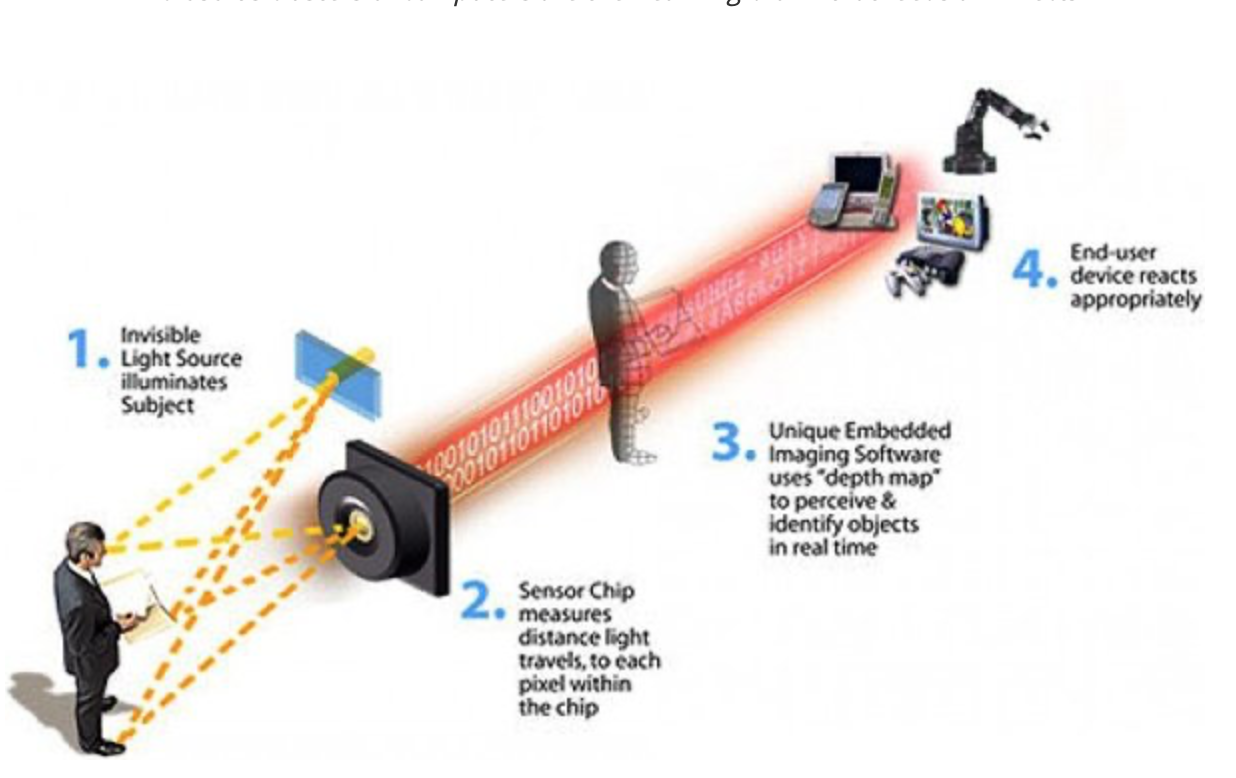
\includegraphics[width=1.0\textwidth]{IDD_LauraMartin_R00124705/Figures/infared.png}
\caption{Explanation of Infrared}
{here goes expl}
\end{figure}



\begin{figure}[h]
\centering
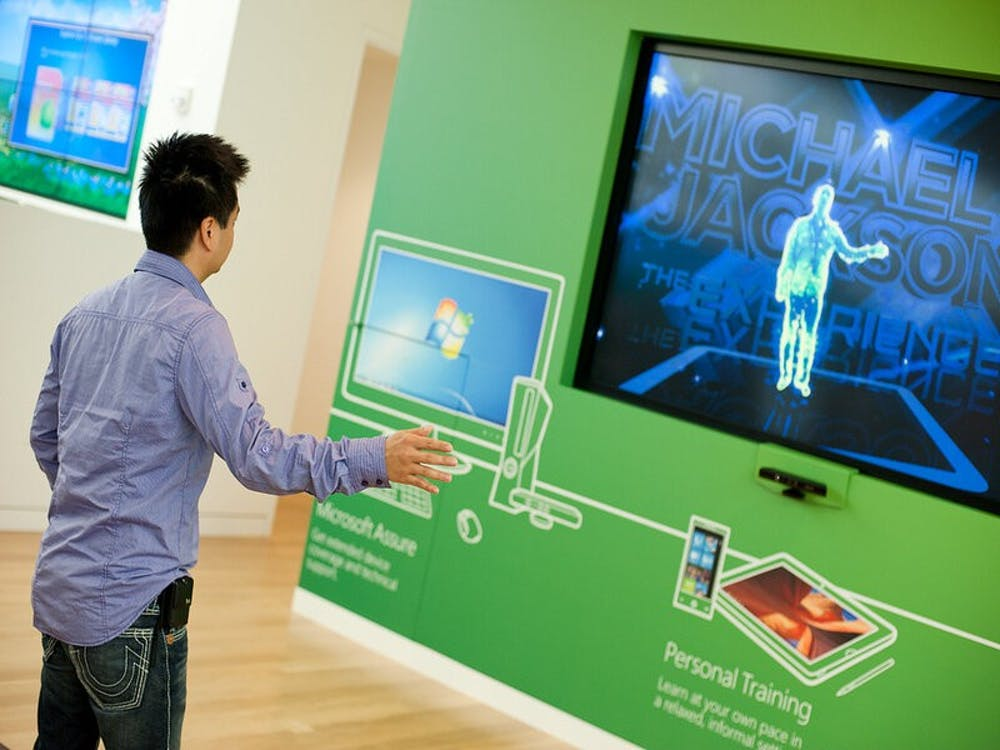
\includegraphics[width=0.5\textwidth]{IDD_LauraMartin_R00124705/Figures/kinect.jpg}
\caption{Kinect in use}
{here goes expl}
\end{figure}

The below images summerise the above images ccccc
figure 3.2 cccc
figure 

\subsection{Existing Design}
The problem with existing information and research that is available is that it requires a physical book or QR code, also known as marker AR to work and that is not always practical. The other problem is that the information in existence is to help a Child with ASD develop to function in a society for individuals who are non-Autistic or considered typical, existing applications teach a Child with ASD to be judged based on facial expressions, for example the paper spoken about earlier and the application Emotrain which is a facial expression recognition tool that judges a Child with ASD and their ability to show emotion and how to react in society and when communicating with other people. This can be challenging for an individual with ASD as they are considered to be literal thinkers and find it difficult to be imaginative with other individuals emotions and have difficulties in portraying their own emotions. The application Emotrain is too general and broad and is not individualised to each user who is Autistic, each person has a different set of characteristics and repetitive patterns, even though they may be similar, the patterns and behaviours will not present as the same and will have various triggers. 

Another area of concern from the application Emotrain is the development of ‘Affectiva’ used by the authors and developers of the Emotrain application, the Affectiva development was created for businesses to understand their customers and was also implemented in the Emotrain application. This is a concern because Affectiva was never developed with the Autistic demographic in mind and the process was never adapted or improved for the use of individuals with Autism, this is an issue due to the Affectiva functionality being too broad and general and not individualised [X]. The consequences of this problem if not resolved are the Autistic users using an application that is not targeted towards them and may have difficulty understanding the application. Another application targeted towards children with autism is 'TaLNA', this application is based on improving the users understanding of basic numeral literacy and calculations. This application claims to boost the child's engagement to learn, to memorise and to recognise numbers through the animated and interactive learning processes. The problem with this application is that it is very narrow and is only targeted to autistic individuals who have difficulty with numeracy comprehension. [X]


The solution this paper and prototype proposes is to develop a markerless AR application, designed through the analysis of existing information, surveys, interviews and prototype testing on applicants with Autism, a parent/guardian of the applicant and Autism educational professionals. It will be an application designed for individuals with Autism and learning disabilities to help them to progress with their academic studies through gamification, AR and AI functionalities. This proposed design will cover all aspects of the educational program taught.

\subsection{Problem Definition}
The problems seen in the market of applications aimed towards children with autism is the user interface is that there are limited guidelines for the user interface (UI) of an applications for children with autism. The design in existing applications is unexplored and unproven and can make the experience for the child with autism increasingly more difficult than it needs to be. A study has been conducted as to what are the main usability factors to consider when design a mobile applications for children with autism. The study researched 23 recent works that followed a set of 6 usability factors, those factors were;

\begin{itemize}
  \item Easy to use
  \item Effectiveness
  \item Understandable
  \item Satisfaction
  \item Appearance
  \item Efficiency
\end{itemize}

 \begin{figure}[h]
\centering
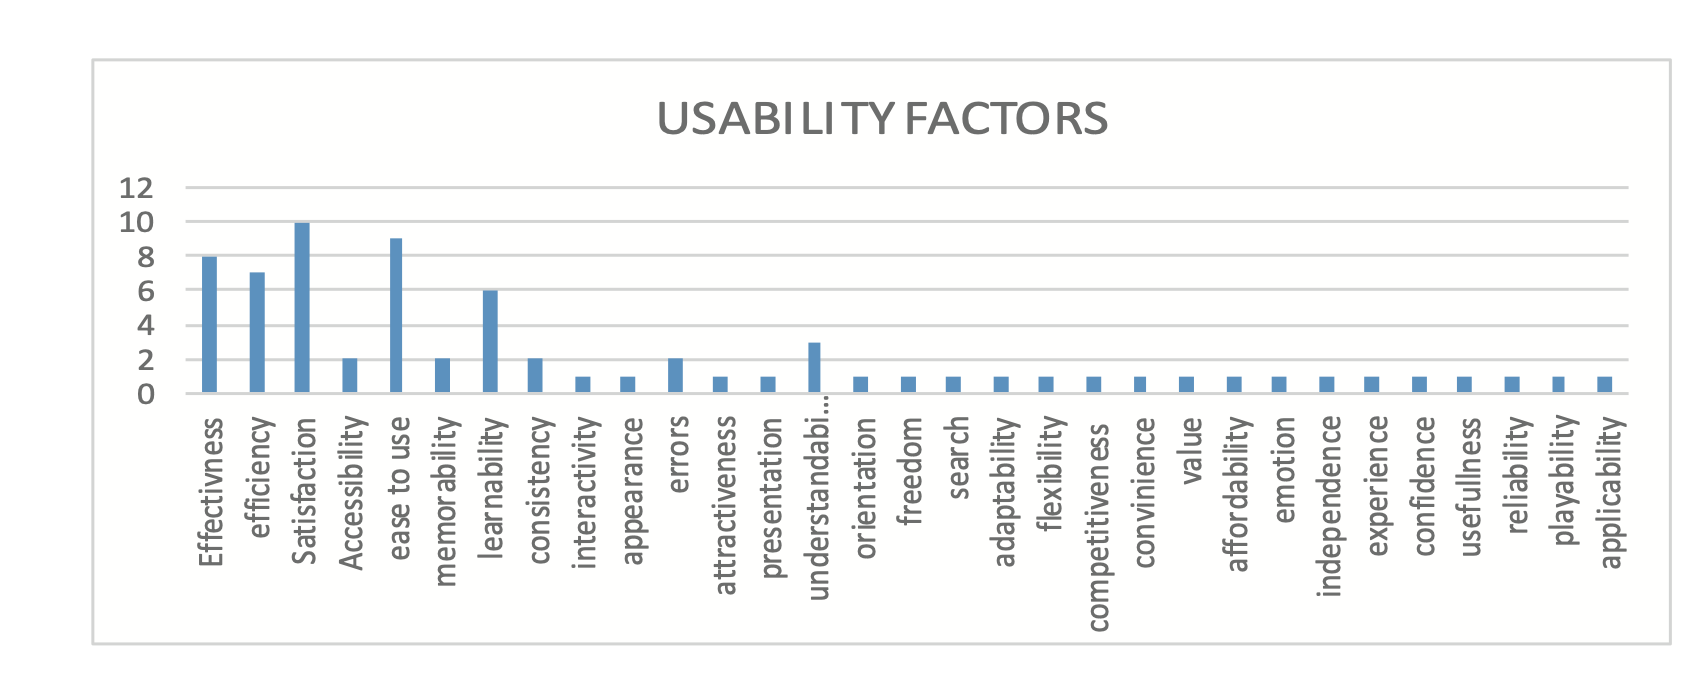
\includegraphics[width=1.0\textwidth]{IDD_LauraMartin_R00124705/Figures/usabilityfactors.png}
\caption{Usability factors}
\end{figure}

To summarise the above figure (figure 3.1), 31 design elements have been identified in the [X] research paper. These elements identify the requirements to be met when designing a mobile application to make it as effective and efficient as possible. 

The problem defined with existing applications outlined in section 3.0.3 is that the existing applications are either too broad, meaning it is not designed for children with autism, but is designed for those who have typical behaviours and patterns. The other problem is the applications being too narrow, meaning the application only covers one area of difficulty, more applications will be needed for the other problem areas, therefor different design and a non-consistent experience for the user.


\subsection{Augmented reality effectiveness in design}
This chapter should include the most relevant/important code listing and discuss relevant/interesting aspects; explain features you wish to highlight. 

\subsection{AI Effectiveness in design}


 

%Provide a high level view of the system and then break down the system. Include any packages or components you are using (the versions of these should be given) and what they are responsible for and what they communicate to. You need to be as specific here as you can. If you have a hardware element in your project this is also where you provide a high level view of how these elements integrate into the project. So for a project that is cyber-physical you will have both a hardware and software architecture diagram.


 % Problem Analysis and Design
\chapter{Research Methodology}
\label{chap:Research Methodology}
\lhead{\emph{Research Methodology}}

\section{Research Methodology}
This research methodology will use both qualitative and quantitative methods 
for analysing. There will be two surveys carried out online to get varied feedback. The first survey will be for educational professionals who educate Children with Autism. The second survey conducted online will be for individuals who have family members, themselves, who have close contact or Child who is Autistic. It is vital to get feedback from both educational professionals and non-educational professionals concerning their understanding of how applications with artificial intelligence and augmented reality can educate children with Autism and other learning disabilities. The first survey, "Professional Educator Survey", will consist of 30 questions for identifying careers and ranks among the participants, their previous knowledge of AR and AI, how technology is used in the class and questions about students ability and possible limitations when it comes to resources available in the school to use technology in the classroom. The second survey, "Autism and Assistive Technology," will have participants who are not educational professionals; they have a personal relationship with a Child with Autism. It is essential to get feedback from individuals with no teaching background or experience; this feedback can be used to design the prototype so the application can be used both for schoolwork and homework.


There will be interviews with three individuals from the educational professionals, two special need teachers and one special needs assistant on the proposed prototype design created in Adobe Illustrator. In conjunction, there will be three interviews with Parents who have a primary school child who is Autistic on the proposed prototype and to gain feedback on the design to make it user friendly for both educational professionals and non-educational professionals. There will be multiple interviews and surveys to get a varying amount of information and feedback on the prototypes and how they can be improved and then implemented into a person with Autism and their education. A person with Autism can have different patterns and behaviours to another person with Autism; it is essential to get feedback from a sample that ranges in age, demographic and employment within the professional educator sector. In order to compare and gain more insight into the topic of AR and AI, existing information from journals, surveys and online content will also be researched and included in this paper. Concerning the information being sourced online, there will have to be things to consider, such as; date range, credibility, sample size being surveyed, and tested. The date range will be significant as more recent information is needed for accurate results due to ongoing upgrades and new products being introduced in technology and education of Children with ASD. Discourse analysis will have to be considered, as looking at communication and meaning (languages, images, non-verbal interactions) will be taken into account for social context.

A custom-built AR filter using Spark and a 3D modelling software will be used in five participants, both males and females with Autism, these participants will be of school-going age, and their abilities will be different to one another. This testing will include two non-verbal Children with Autism. They are currently being introduced to other communication learning applications in their school and home to help with their current communication difficulties. Finally, for prototype testing, a short demo video of the proposed design will be created in After Effects and shown to both participants who were involved in the interviews, the parents from the surveys who have a Child with Autism and the Autistic individuals to get feedback and to be able to analyse results.




The following will be taken into consideration during testing.
\begin{itemize}
    \item Control - The same number of activities and time will be given to each participant. 
    \item Sample Size - The sample size will include both males and females; the participants will vary in age and demographics.
    \item Replicates - The same experiment will be given to each sample of participants depending on their severity of the disability.
\end{itemize}

Participants will be found through an ASD unit; all Autistic participants will be of school-going age as this is a formal operational stage for typical Children. School going age in typical children can use logic to solve problems, view the world around them, and plan. [6]. Groups will be small due to a lack of access to a large group of Children with Autism and this will give precise and accurate information for the data analysis. When all surveys, interviews and testing has been conducted, there will be a section for analysis on the results and a conclusion of the research findings. 

While conducting user interviews and user testing to develop standard operating procedures (SOPs) that will align with the proposed design.  Interviews will be based on questions to determine what key  design  factors are beneficial to the proposed application while  using  an  SOP  and  how  they  perceive their performance  while interacting with an SOP. % Implementation
\chapter{Survey one results and analysis}
\label{chap:Survey one results and analysis}
\lhead{\emph{Survey one results and analysis}}
This chapter will show the visuals of the results from both surveys conducted, the first section will be the professional educator survey results and the second survey will be the Autism and Assistive Technology Survey. Each survey will be followed by a table to give overall and interesting feedback from the respective survey conducted.

\section{Survey one results}

Survey one  is the professional educator Survey, this survey involved 24 participants who all had experience educating individuals with Autism. The participants occupations included home educator, special needs teacher, speech and language therapist, additional needs educator and various other professional educator roles.

\begin{figure}[ht]
\centering
\includegraphics[width=1.0\textwidth]{IDD_LauraMartin_R00124705/Figures/1.png}
\caption{Occupation answer box }
{For question one, 24 participants best described their occupation in the field of professional education.}
\end{figure}

\begin{figure}[ht]
\centering
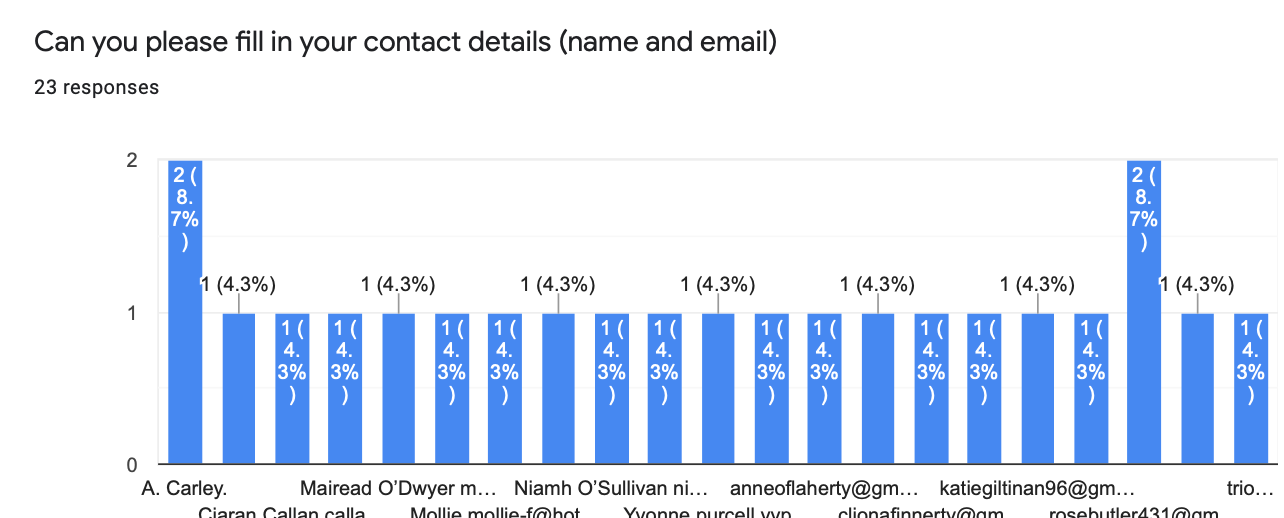
\includegraphics[width=1.0\textwidth]{IDD_LauraMartin_R00124705/Figures/2.png}
\caption{Details of participants}
{For question two, 23 respondents gave their name and email addresses.}
\end{figure}

\begin{figure}[ht]
\centering
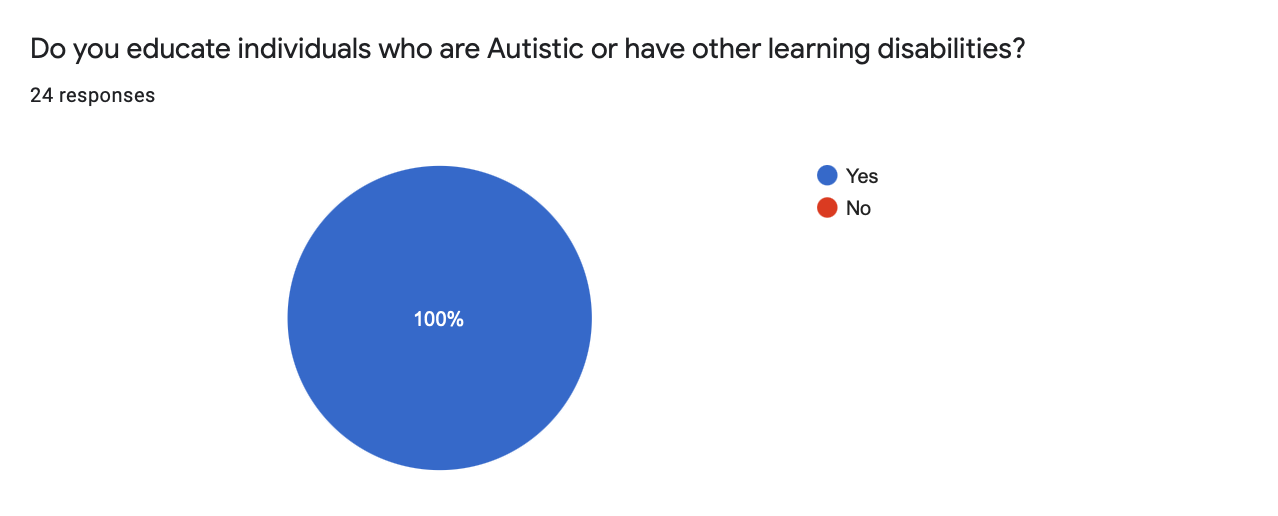
\includegraphics[width=1.0\textwidth]{IDD_LauraMartin_R00124705/Figures/4.png}
\caption{Pie chart representing the participants involvement of educating individuals with Autism}
{For question three, 24 respondents gave their experience educating individuals with Autism.}
\end{figure}

\begin{figure}[ht]
\centering
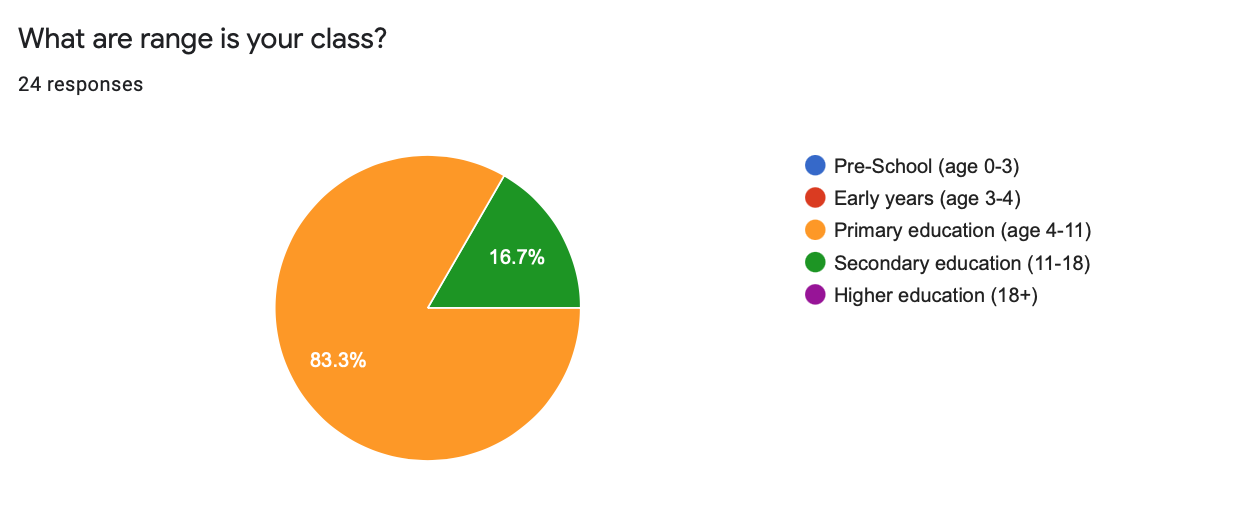
\includegraphics[width=1.0\textwidth]{IDD_LauraMartin_R00124705/Figures/5.png}
\caption{Pie chart representing the participants class age range}
{For question four, 24 respondents gave the age range of their class, age 4-11 being the most popular age range and followed by 11-18 years old.}
\end{figure}

\begin{figure}[ht]
\centering
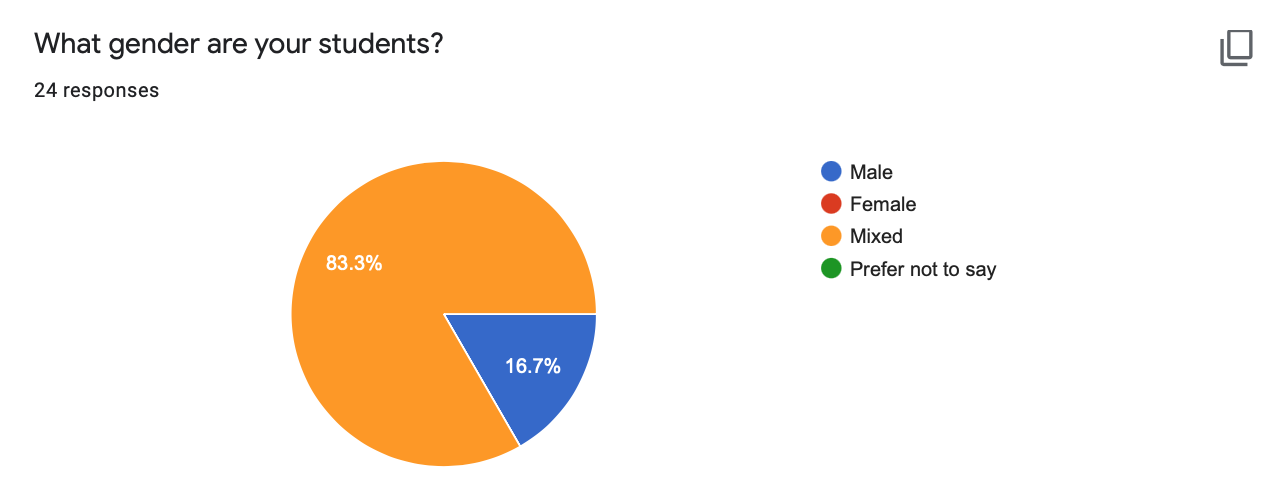
\includegraphics[width=1.0\textwidth]{IDD_LauraMartin_R00124705/Figures/6.png}
\caption{Pie chart representing the participants genders in their classroom}
{For question five, 24 respondents gave the gender of the students they had in the classroom, mixed being the most popular answer, followed by a full male classroom.}
\end{figure}

\begin{figure}[ht]
\centering
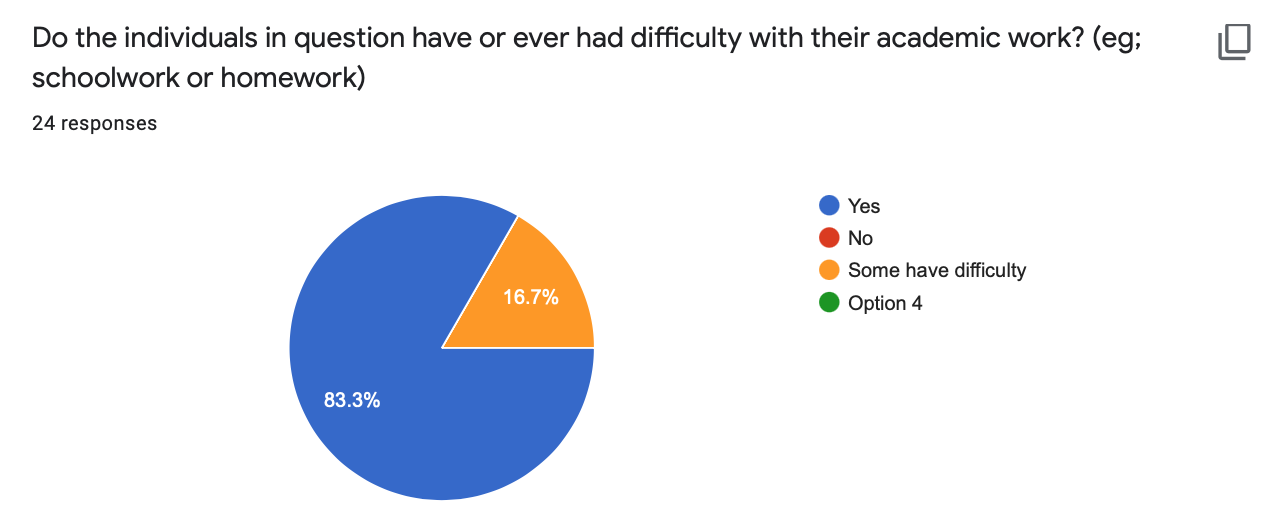
\includegraphics[width=1.0\textwidth]{IDD_LauraMartin_R00124705/Figures/7.png}
\caption{Difficulty with academic studies pie chart}
{for question six, 24 respondents were given a multiple choice question about their students having difficulty with academic studies.}
\end{figure}

\begin{figure}[ht]
\centering
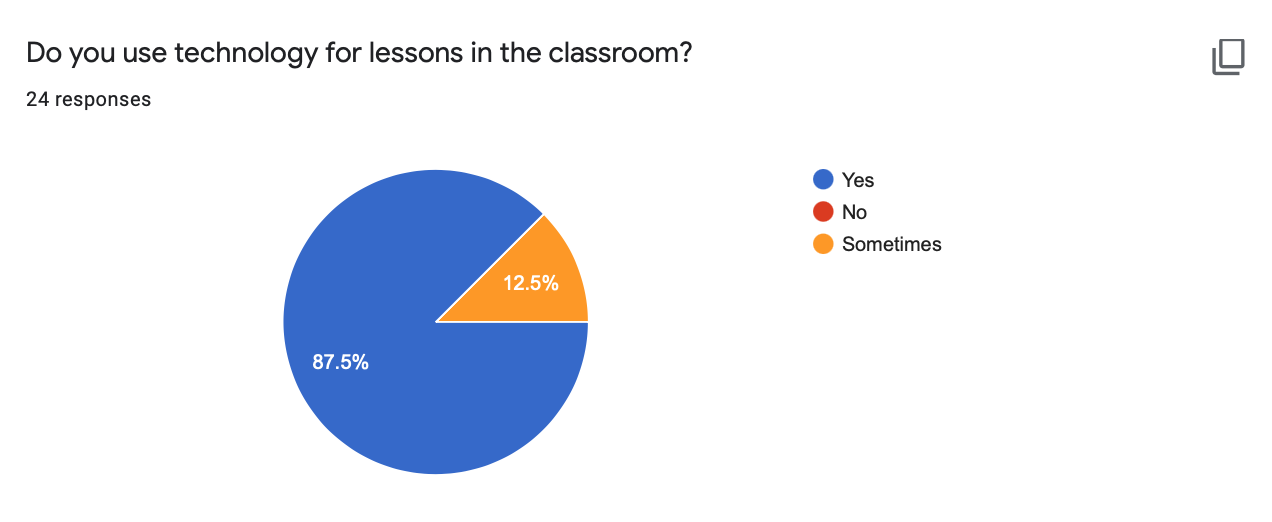
\includegraphics[width=1.0\textwidth]{IDD_LauraMartin_R00124705/Figures/8.png}
\caption{Pie chart representing the participants relationship with a person with Autism.}
{For question six, 24 respondents answered was technology used in the classroom, the highest response was yes at 87.5 percent and sometimes at 12.5 percent.}

\end{figure}

\begin{figure}[ht]
\centering
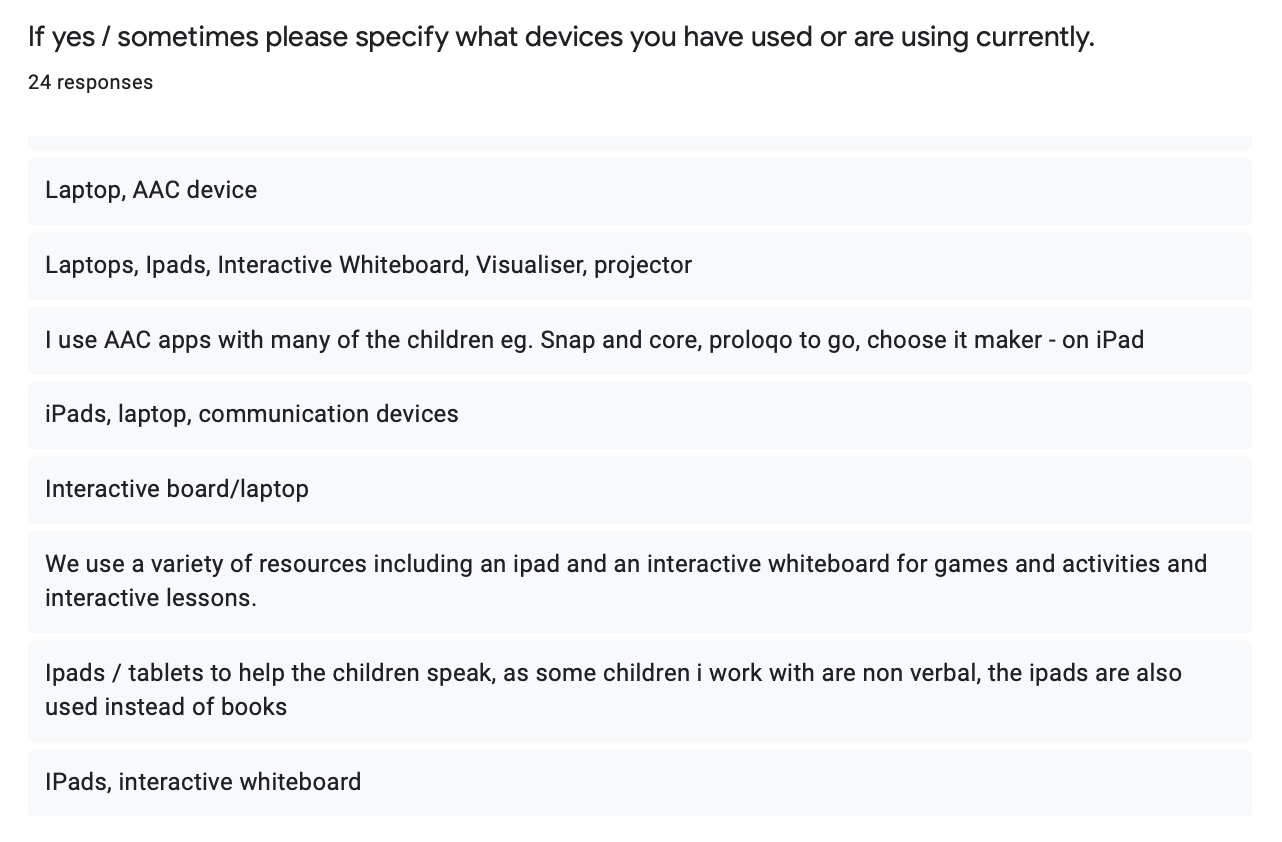
\includegraphics[width=1.0\textwidth]{IDD_LauraMartin_R00124705/Figures/9.png}
\caption{Technology and individuals in the classroom answer box}
{For question seven, 24 participants specified what technology they used in the classroom.}

\end{figure}

\begin{figure}[ht]
\centering
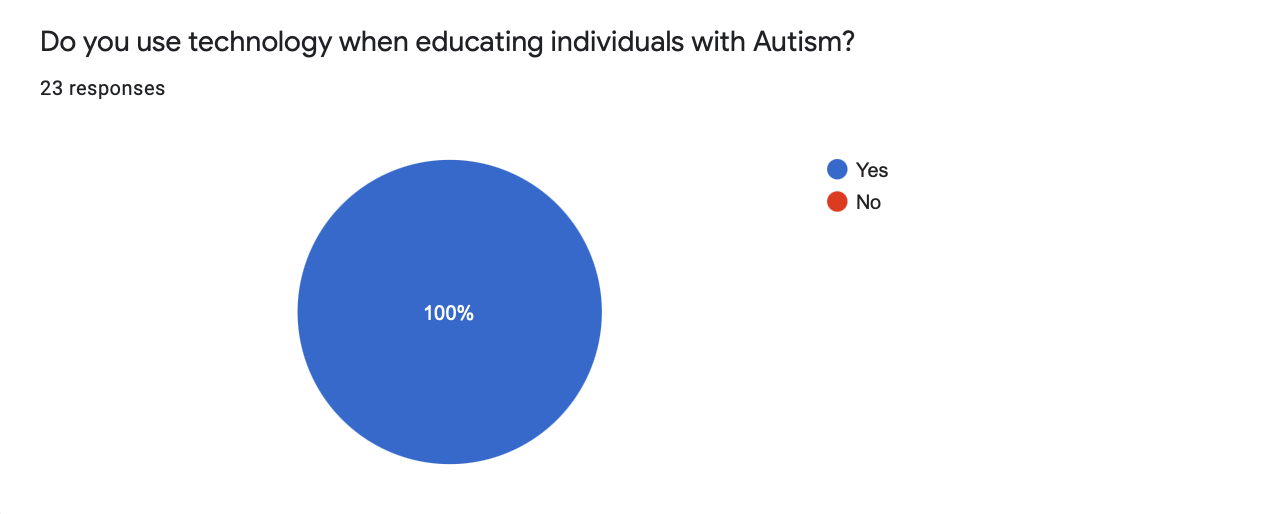
\includegraphics[width=1.0\textwidth]{IDD_LauraMartin_R00124705/Figures/10.png}
\caption{Technology and individuals with Autism pie chart}
{For question eight, 23 respondents answered a multiple choice question asking was technology used when educating individuals with Autism, yes was the response for all participants.}
\end{figure}

\begin{figure}[ht]
\centering
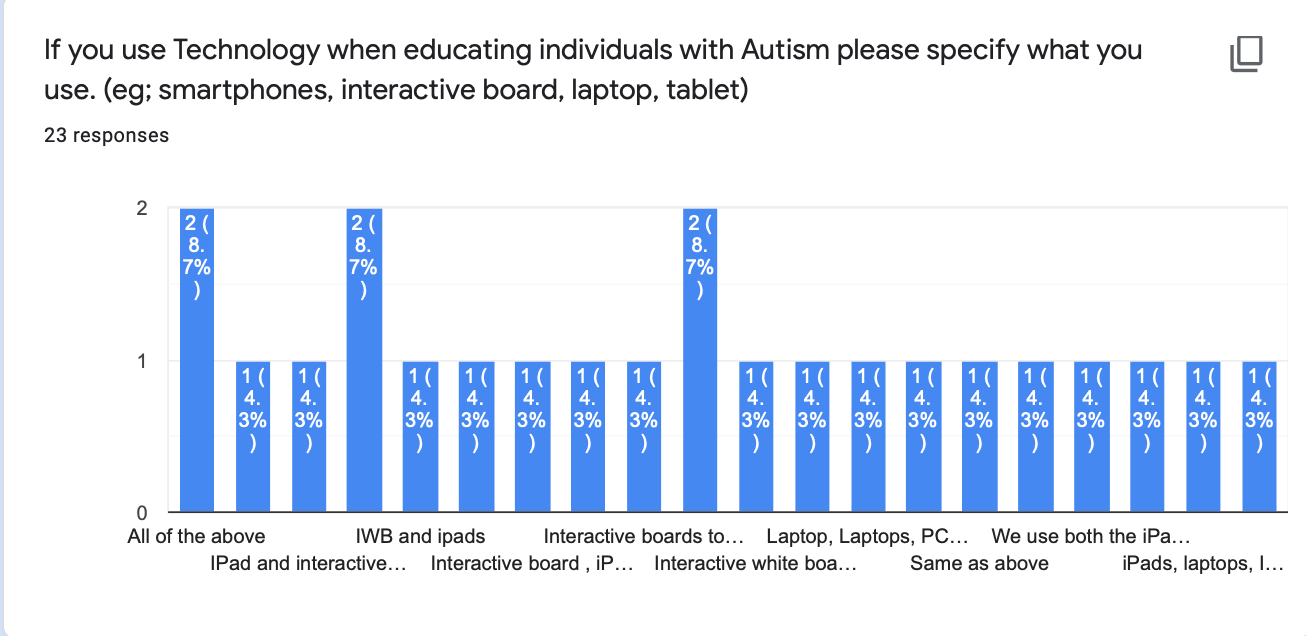
\includegraphics[width=1.0\textwidth]{IDD_LauraMartin_R00124705/Figures/11.png}
\caption{Technology used answer box}
{For question nine, 23 respondents answered what what technology they used when educating a student with Autism.}
\end{figure}

\begin{figure}[ht]
\centering
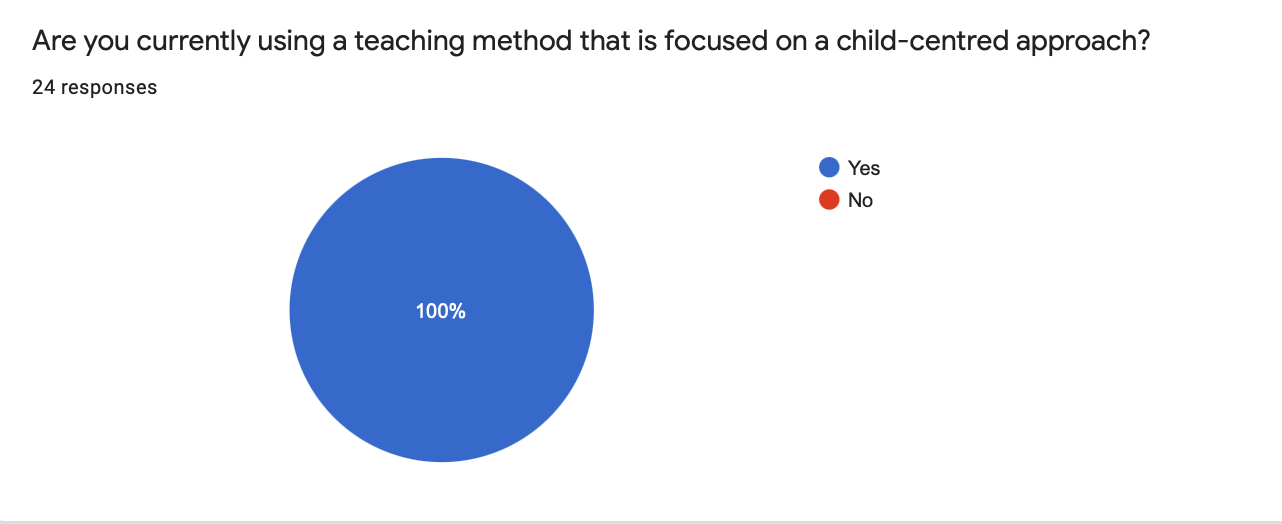
\includegraphics[width=1.0\textwidth]{IDD_LauraMartin_R00124705/Figures/12.png}
\caption{Child centered approach pie chart}
{For question ten, 24 respondents were asked if they used a child centered approach in the classroom, all participants answered yes.}
\end{figure}

\begin{figure}[ht]
\centering
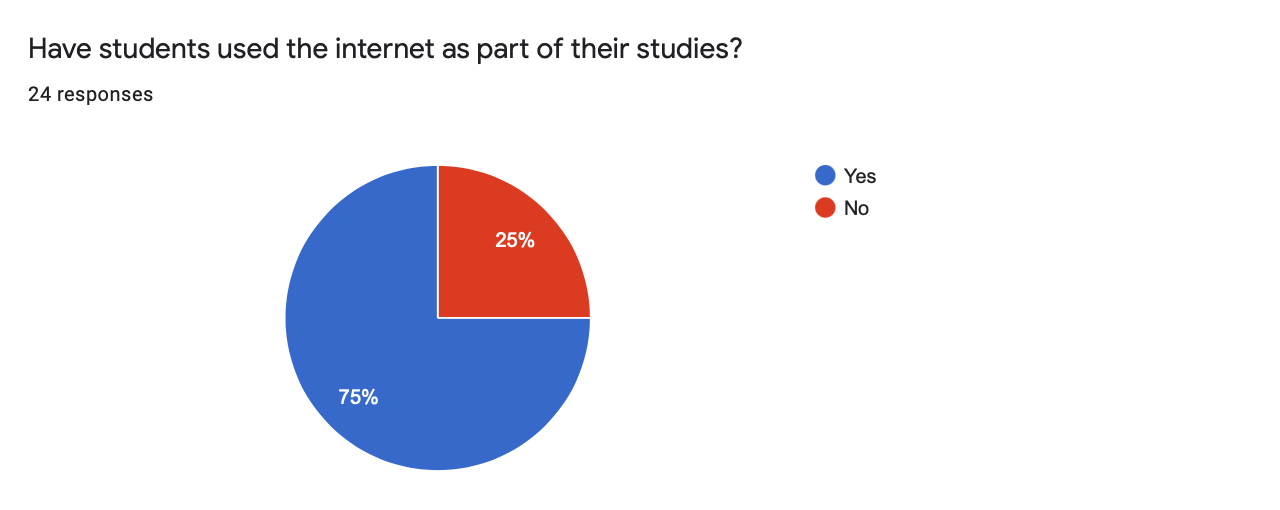
\includegraphics[width=1.0\textwidth]{IDD_LauraMartin_R00124705/Figures/13.png}
\caption{Students using the internet as part of studies pie chart}
{For question eleven, 24 respondents were given a multiple choice question asking if they used the internet as part of their studies, 75 percent answered yes and 25 percent answered no.}
\end{figure}

\begin{figure}[ht]
\centering
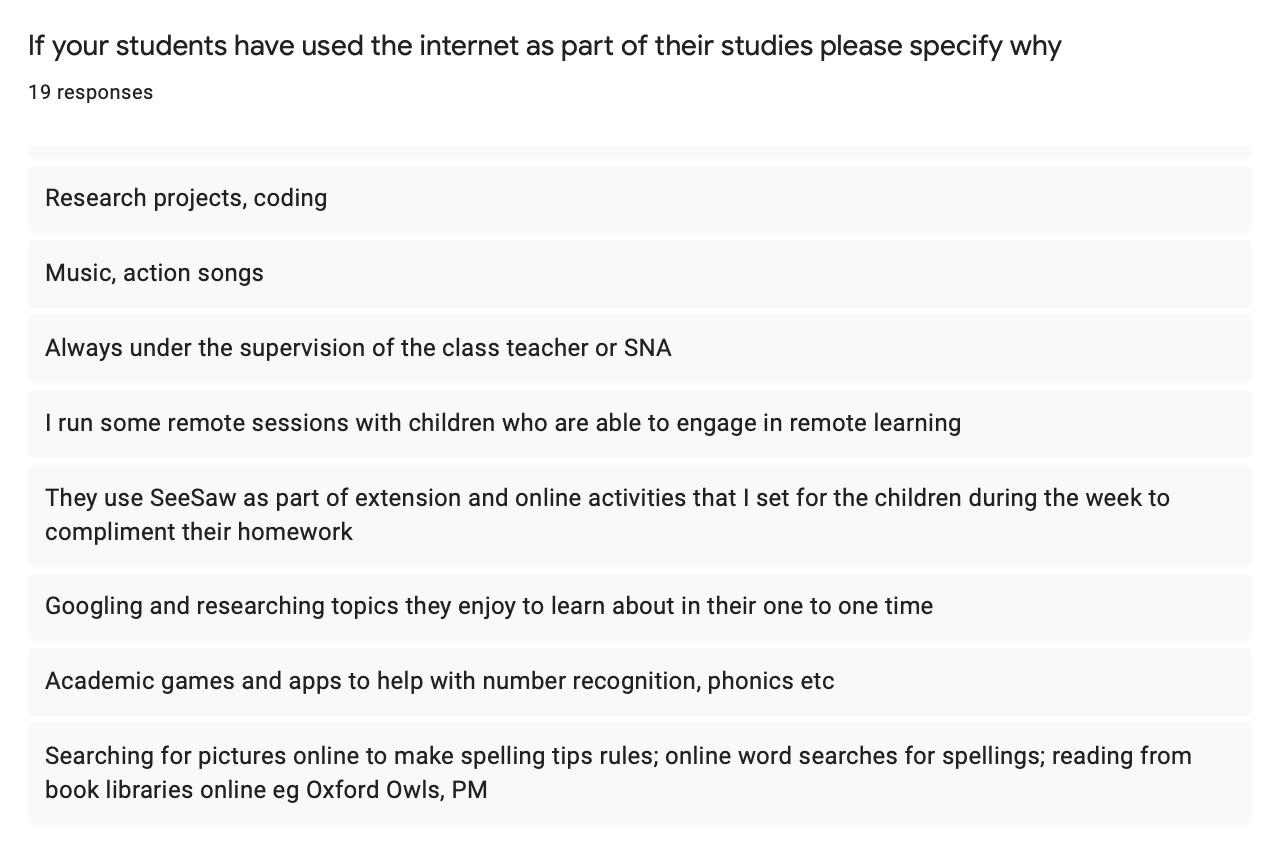
\includegraphics[width=1.0\textwidth]{IDD_LauraMartin_R00124705/Figures/14.png}
\caption{Internet used for studies answer box}
{For question Twelve, 19 respondents details on why their students use the internet as part of their studies.}
\end{figure}

\begin{figure}[ht]
\centering
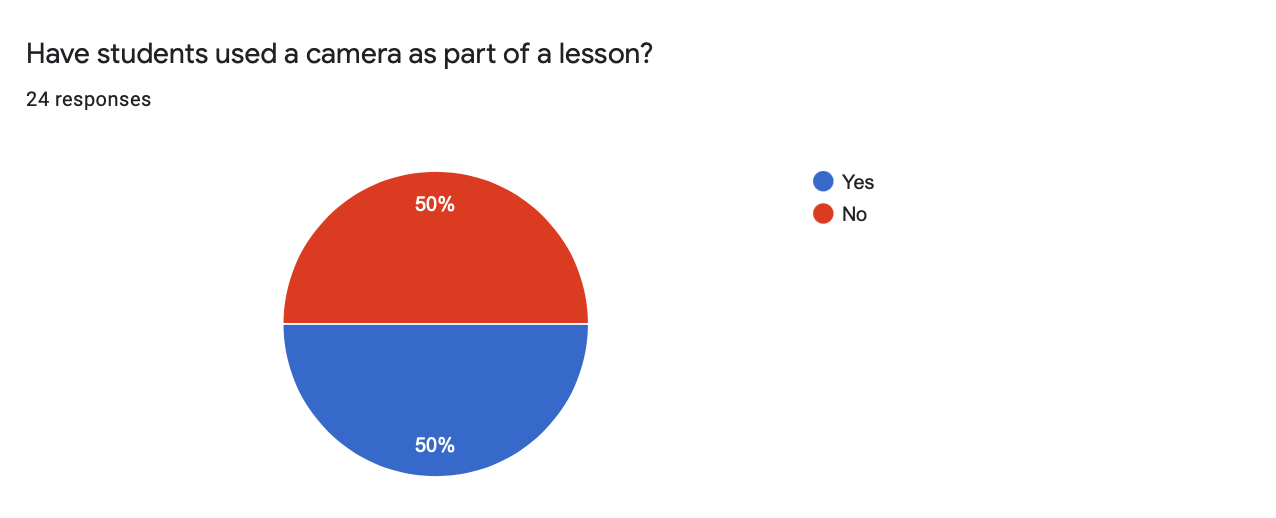
\includegraphics[width=1.0\textwidth]{IDD_LauraMartin_R00124705/Figures/15.png}
\caption{Smartphone camera used during lessons pie chart}
{For question thirteen, 24 respondents answered is their students used a camera as part of a lesson, 50 percent said yes and 50 percent said no.}
\end{figure}

\begin{figure}[ht]
\centering
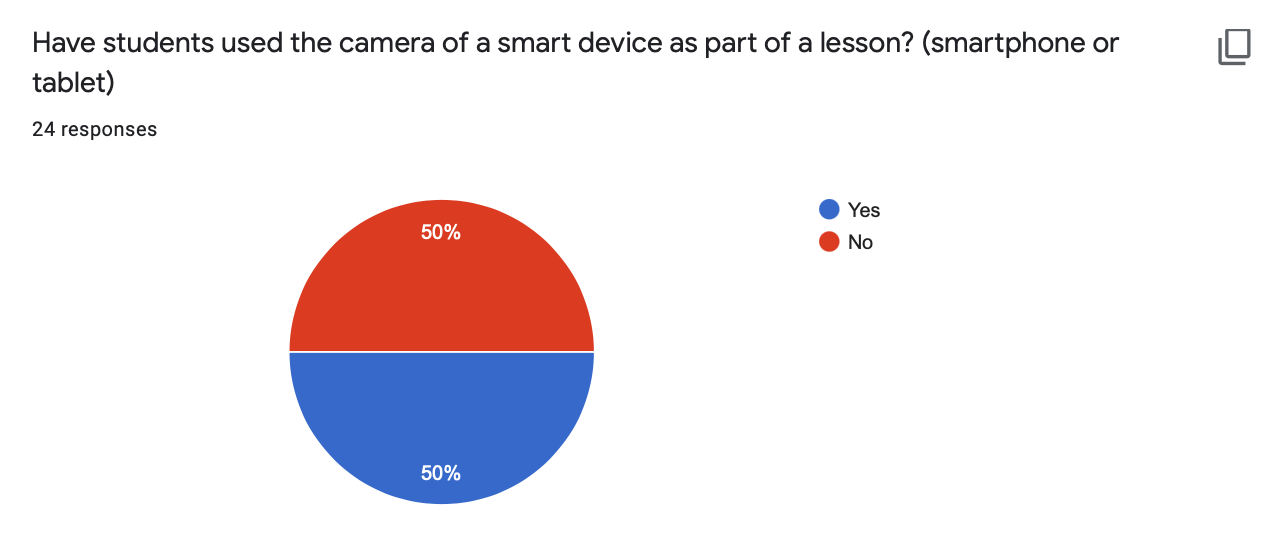
\includegraphics[width=1.0\textwidth]{IDD_LauraMartin_R00124705/Figures/16.png}
\caption{Use of a camera on a smart device during lessons pie chart}
{For question thirteen, 24 respondents answered is their students used a smartphone camera as part of a lesson, 50 percent said yes and 50 percent said no.}
\end{figure}

\begin{figure}[ht]
\centering
\includegraphics[width=1.0\textwidth]{IDD_LauraMartin_R00124705/Figures/17.1.png}
\caption{Why have students used a camera on a smart device during lessons answer box}
{For question fourteen, 13 respondents answered why a student used a smartphone camera as part of a lesson.}
\end{figure}

\begin{figure}[ht]
\centering
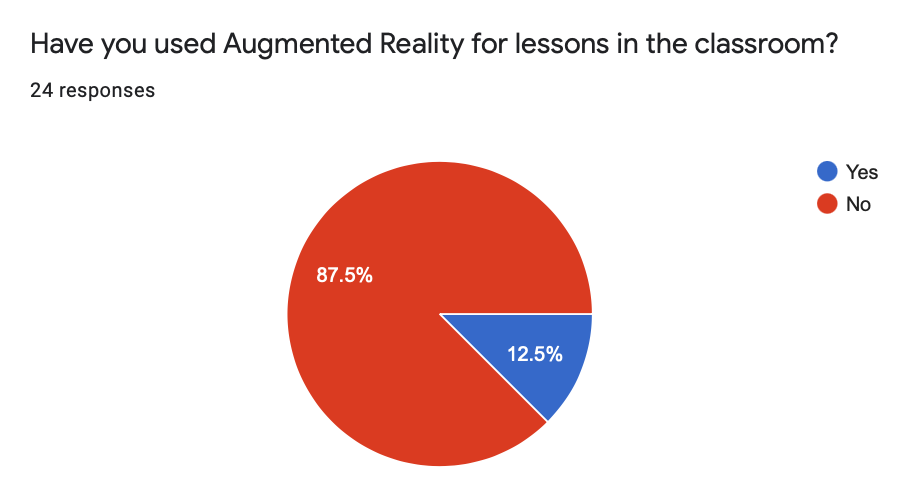
\includegraphics[width=1.0\textwidth]{IDD_LauraMartin_R00124705/Figures/17.png}
\caption{Use of AR in the classroom pie chart}
{For question fifteen, 24 respondents answered if they used AR for lessons in the classroom, 87.5 percent said no and 12.5 percent said yes.}
\end{figure}

\begin{figure}[ht]
\centering
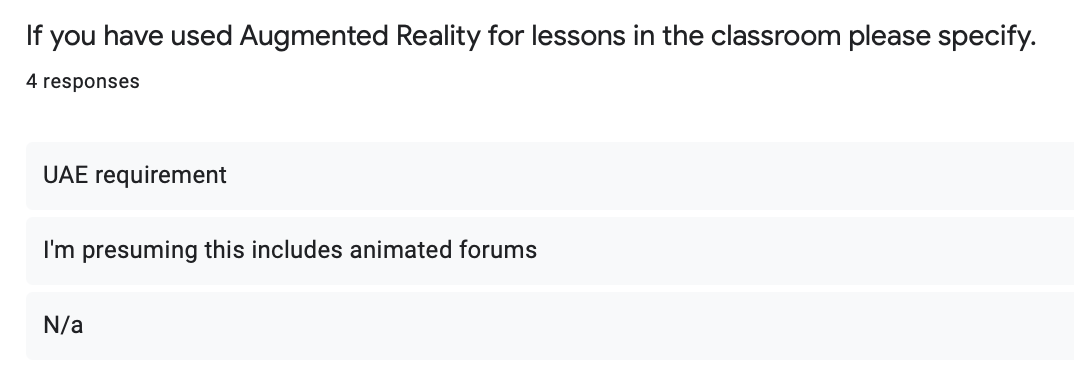
\includegraphics[width=1.0\textwidth]{IDD_LauraMartin_R00124705/Figures/18.png}
\caption{Use of AR in the classroom answer box}
{For question sixteen, 4 respondents explained why they have used AR in the classroom.}

\end{figure}

\begin{figure}[ht]
\centering
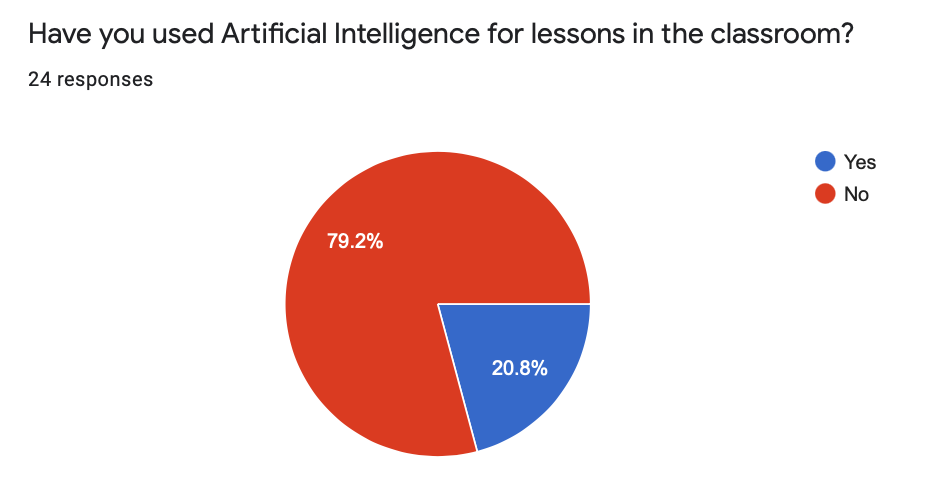
\includegraphics[width=1.0\textwidth]{IDD_LauraMartin_R00124705/Figures/19.png}
\caption{Use of AI pie chart}
{For question seventeen, 24 respondents answered if they used AI for lessons in the classroom, 79.2 percent said no and 20.8 percent said yes.}
\end{figure}

\begin{figure}[ht]
\centering
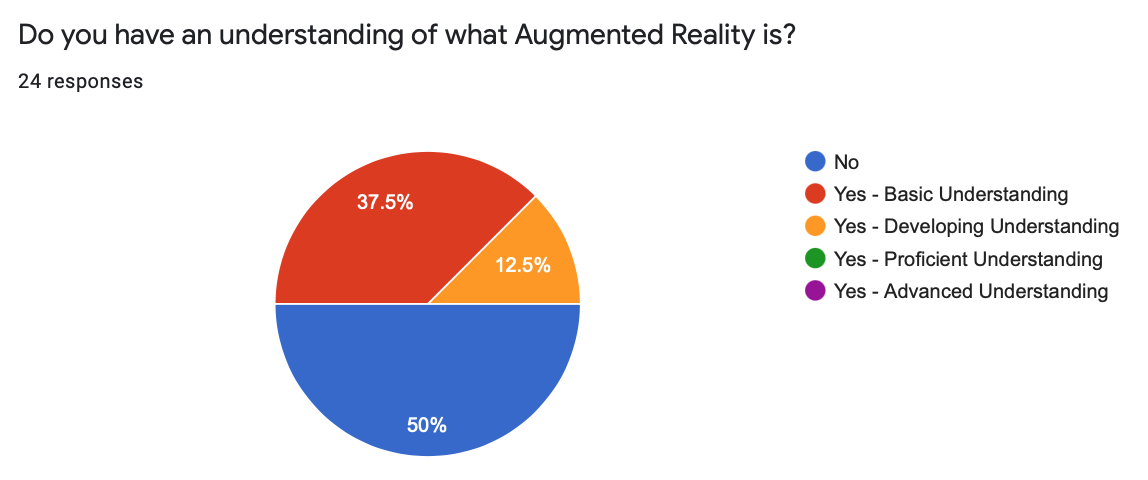
\includegraphics[width=1.0\textwidth]{IDD_LauraMartin_R00124705/Figures/20.png}
\caption{Participants understanding of AR pie chart}
{For question eighteen, 24 respondents were asked a multiple choice question asking if they had an understanding of AR, 50 percent of participants said no, 37.5 percent said yes and 12.5 percent said they had a developing understanding.}
\end{figure}

\begin{figure}[ht]
\centering
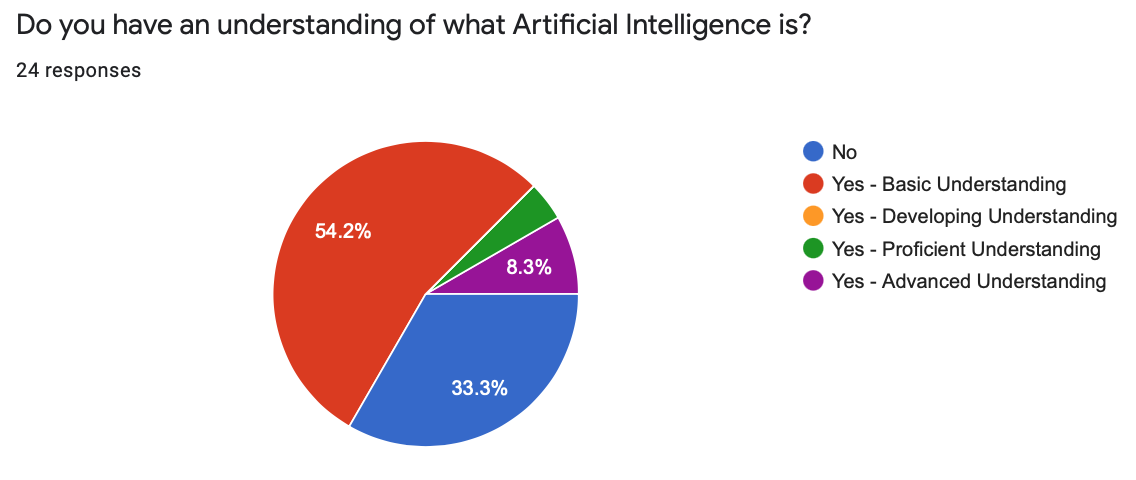
\includegraphics[width=1.0\textwidth]{IDD_LauraMartin_R00124705/Figures/21.png}
\caption{Participants understanding of AI pie chart}
{For question nineteen, 24 respondents were asked a multiple choice question asking if they had an understanding of AI, 33.3 percent of participants said no, 54.2 percent said yes - basic understanding, XX said yes - proficient understanding and 8.3 percent claim to have an advanced understanding of AI.}
\end{figure}

\begin{figure}[ht]
\centering
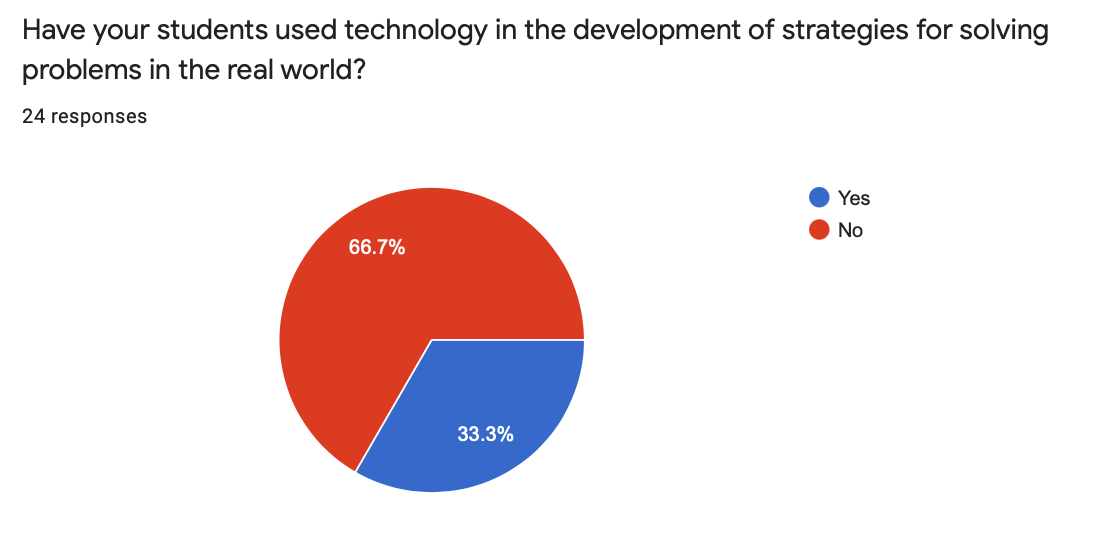
\includegraphics[width=1.0\textwidth]{IDD_LauraMartin_R00124705/Figures/22.png}
\caption{Students use of technology to solve real world problems pie chart}
{For question twenty, 24 respondents were asked if their students used technology to solve real world problems, 66.7 percent saud no and 33.3 percent said yes.}
\end{figure}

\begin{figure}[ht]
\centering
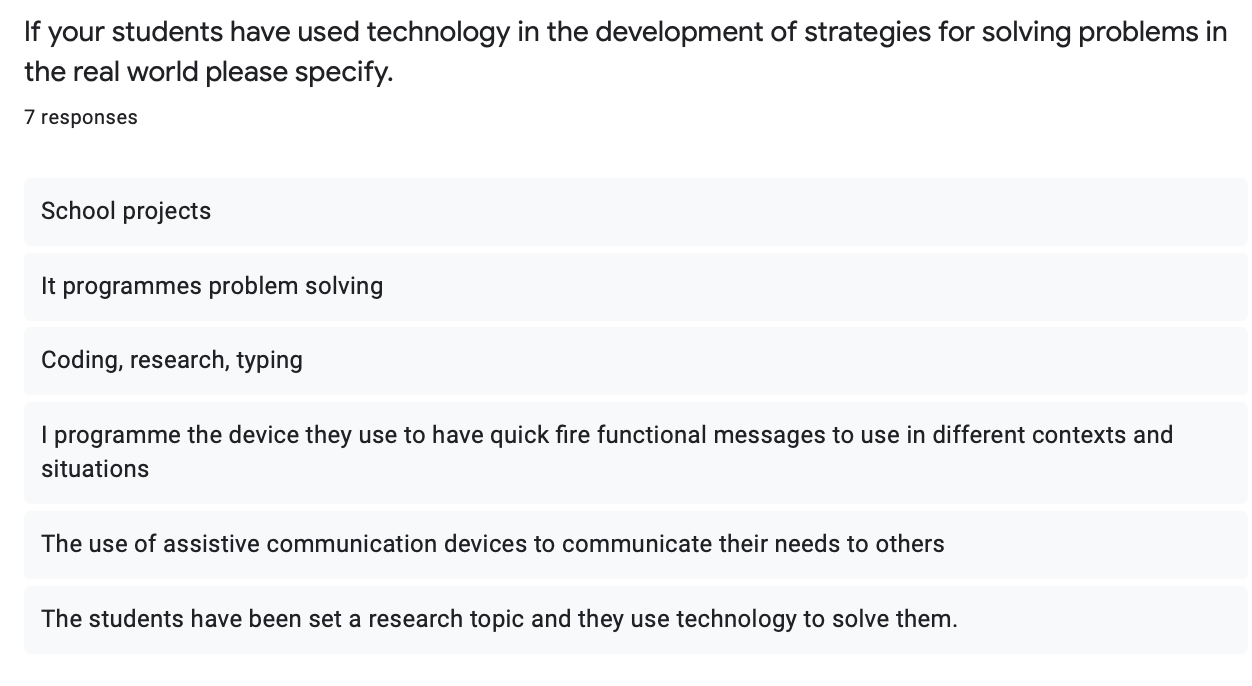
\includegraphics[width=1.0\textwidth]{IDD_LauraMartin_R00124705/Figures/23.png}
\caption{Students use of technology to solve real world problems answer box}
{For question twenty one, 7 respondents explained how their students used technology for real world problems.}
\end{figure}

\begin{figure}[ht]
\centering
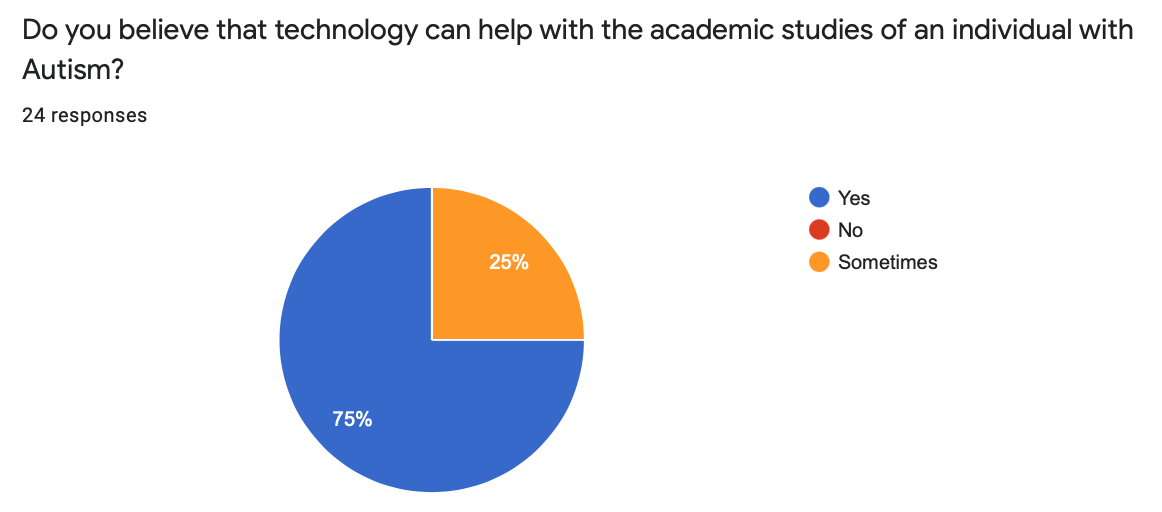
\includegraphics[width=1.0\textwidth]{IDD_LauraMartin_R00124705/Figures/24.png}
\caption{Technology and an Autistic individuals academic studies pie chart}
{For question twenty two, 24 were asked if they believe technology can help with the education of a student with Autism. 75 percent of the participants said yes and 25 percent said sometimes.}
\end{figure}

\begin{figure}[ht]
\centering
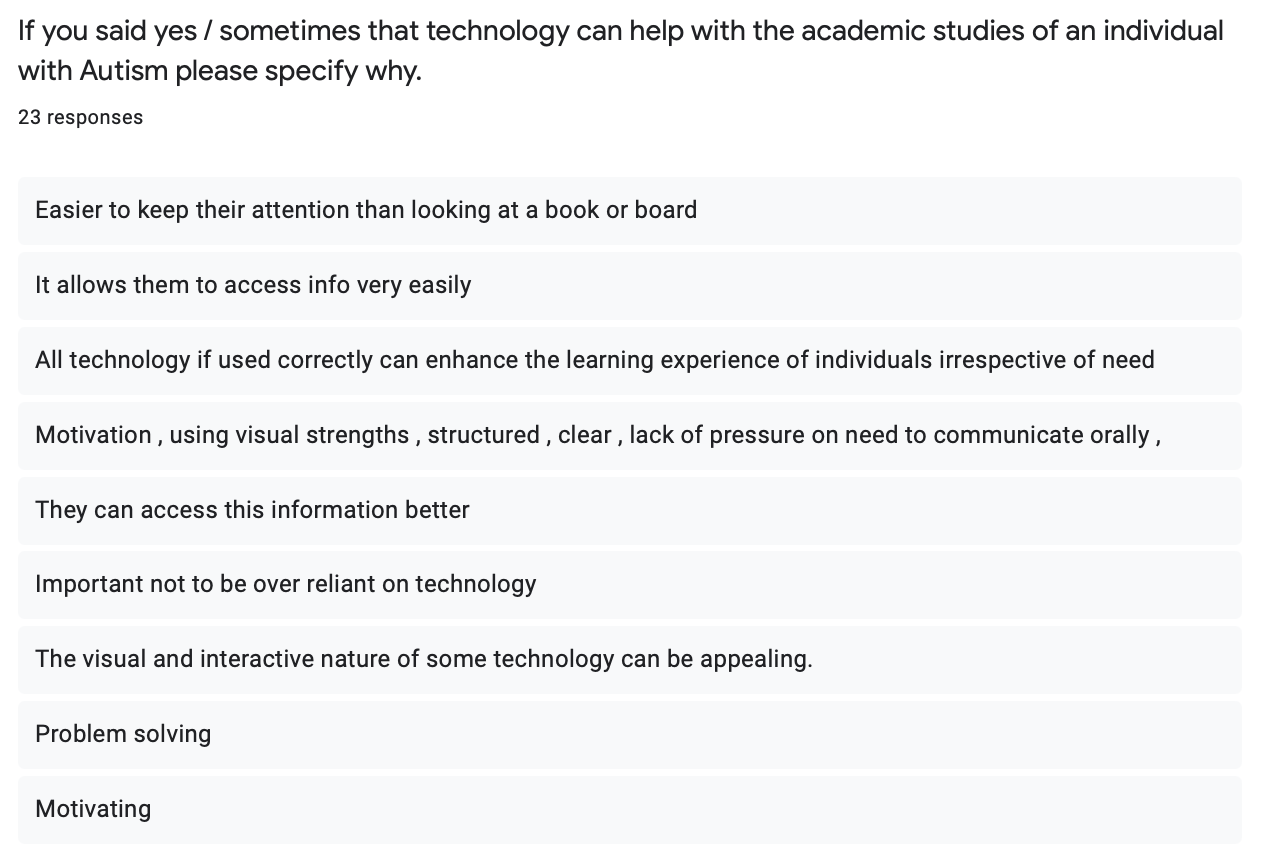
\includegraphics[width=1.0\textwidth]{IDD_LauraMartin_R00124705/Figures/25.png}
\caption{Technology and an Autistic individuals academic studies answer box}
{For question twenty three, 23 respondents gave feedback on how technology can help with the academic studies of an individual with Autism.}
\end{figure}

\begin{figure}[ht]
\centering
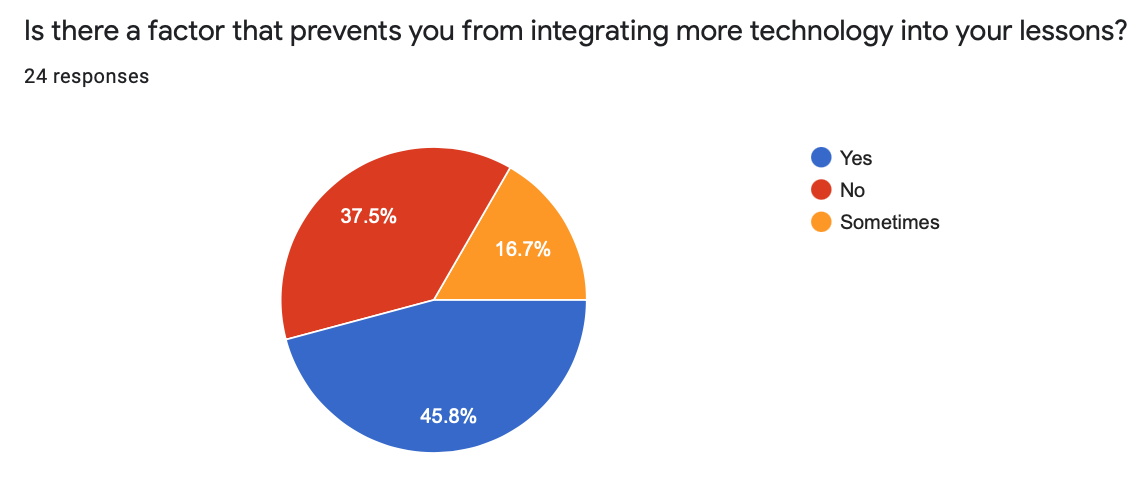
\includegraphics[width=1.0\textwidth]{IDD_LauraMartin_R00124705/Figures/26.png}
\caption{More technology integration pie chart}
{For question twenty four, 24 respondents were asked a multiple choice question of factors that could prevent them from integrating more technology into their lessons. 45.8 percent said yes, 37.5 percent said no and 16.7 percent said sometimes.}
\end{figure}

\begin{figure}[ht]
\centering
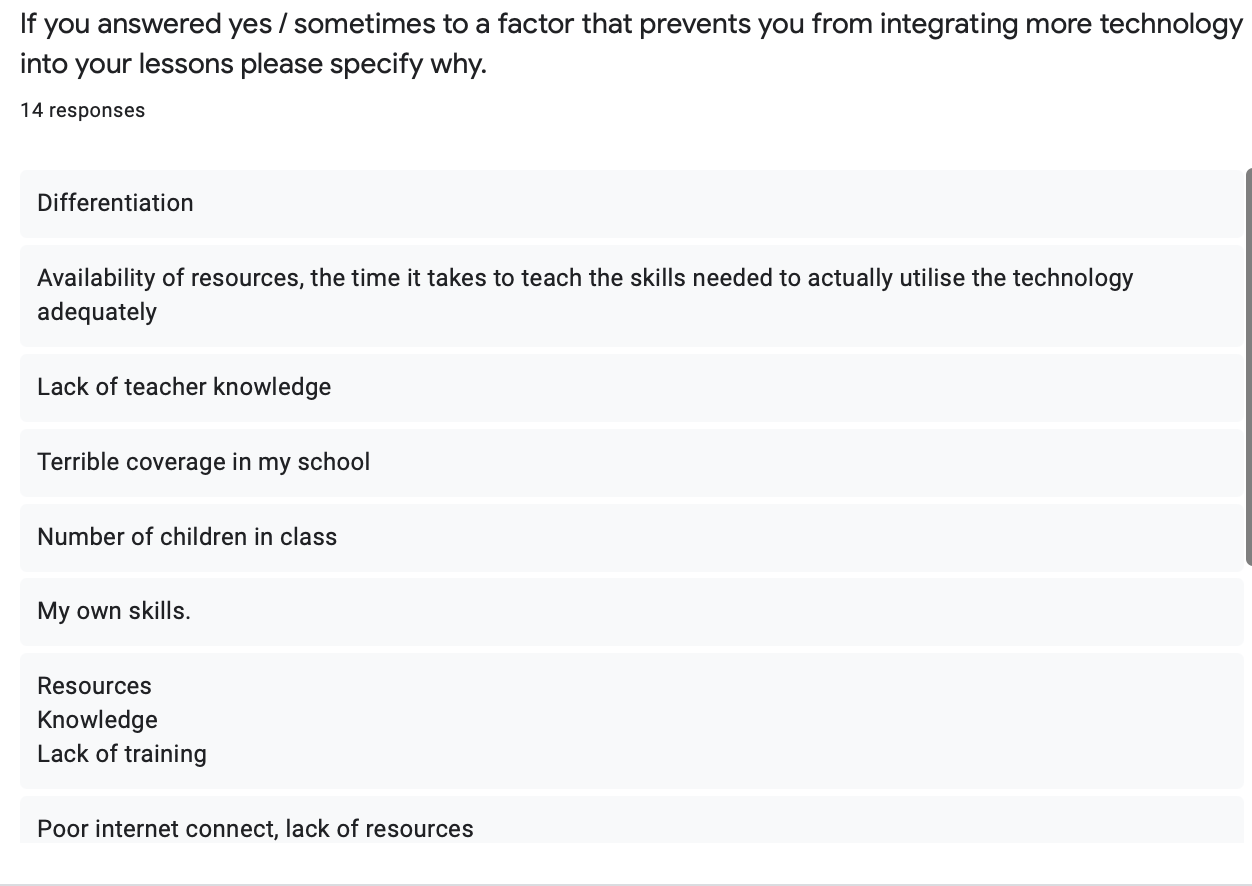
\includegraphics[width=1.0\textwidth]{IDD_LauraMartin_R00124705/Figures/27.png}
\caption{More technology integration answer box}
{For question twenty five, 14 respondents gave information as to why they have or sometimes have factors that prevent them using more technology in their lessons.}
\end{figure}

\begin{figure}[ht]
\centering
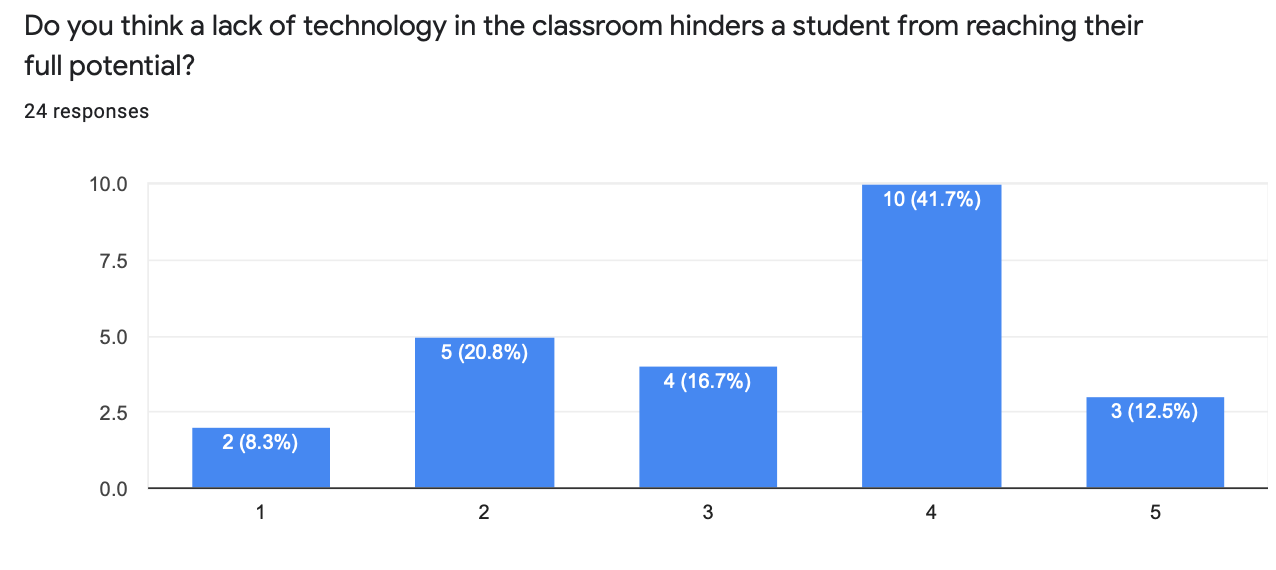
\includegraphics[width=1.0\textwidth]{IDD_LauraMartin_R00124705/Figures/28.png}
\caption{Technology hindering a student from reaching their full potential liner graph}
{For question twenty six, 24 participants answered a linear graph asking do they think a lack of technology can hinder a student reaching their full potential, rank 1 is strongly disagree and rank 5 was strongly agree.}
\end{figure}

\begin{figure}[ht]
\centering
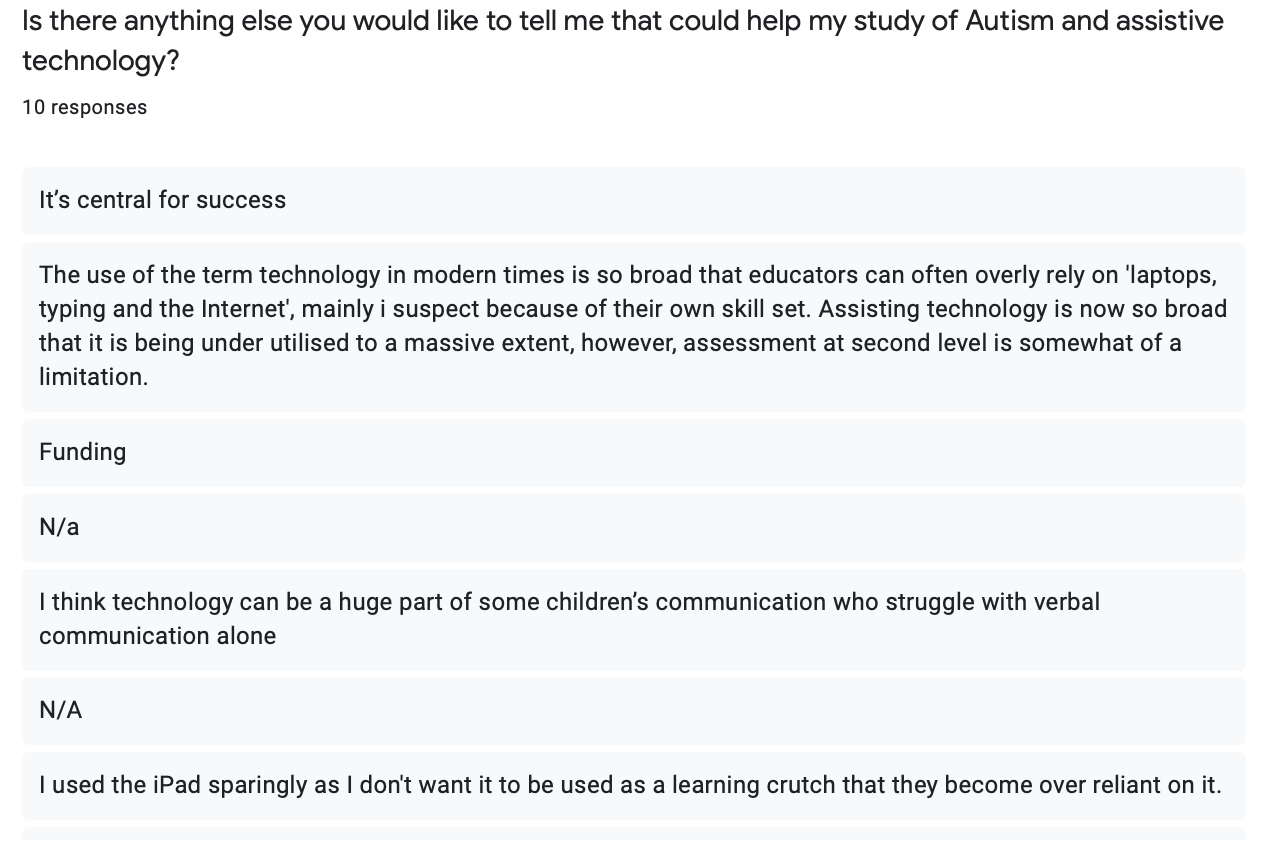
\includegraphics[width=1.0\textwidth]{IDD_LauraMartin_R00124705/Figures/29.png}
\caption{Additional information for this study answer box}
{For question twenty seven, 11 respondents gave feedback that could improve the study going forwards.}
\end{figure}


%\newpage

\subsection{Survey one analysis}

\begin{table} [b]
    \centering
\begin{tabular}{ | m{3em} | m{10cm}| } 
\hline
Q1. & There is a good range of occupations that are related to the target audience. \\ 
\hline
Q.2 & This question gave the details of the participants, it concluded of their name and email address for further contact. \\ 
\hline
Q.3 & 100 percent of the participants educates a person with Autism, this is crucial for feedback and design going foreword.  \\ 
\hline
Q.4 & 83.3 percent of the respondents educated children with Autism who were the school going age of 4-11, this is vital information as that is the age of the demographic for the proposed application.  \\ 
\hline
Q.5 & 83.3 percent of the respondents educated children in a mixed gender school, while 16.7 percent taught in a all male school. This is interesting feedback as none of the applicants educated in an all female school.  \\ 
\hline
Q.6 & 83.3 percent of the respondents claimed their students struggled with either their homework or their school work and 16.7 percent had some difficulty. This result was to be expected as the Children are learning new skills and having a learning disability typically can make this challenging.   \\ 
\hline
Q.7 & 87.5 percent of the participants use technology in the class while 12.5 percent only sometimes use technology, this can be put down to limitations, resources and internet connection in the school. \\ 
\hline
Q.8 & All respondents explained what devices they used in the classroom, the most common answer was a form of tablet and an interactive whiteboard. \\ 
\hline
Q.9 & 100 percent of the respondents used a form of technology for educating students with Autism. \\ 
\hline
Q.10 & The respondents explained what form of devices they used to educate a student with Autism, the most common answer was an interactive whiteboard and a form of table. \\ 
\hline
Q.11 & 100 percent of the respondents used a child centered approach when educating students with Autism, this is expected as it is a recommend form of practice for individuals with Autism as ability can vary. \\ 
\hline
Q.12 & 75 percent of respondents used the internet as part of their studies, while 25 percent did not. This is interesting as due to the COVID-19 pandemic all schools in Ireland for a period of time had to migrate to teaching online. \\ 
\hline

Q.13 & Respondents gave an explanation as to why students would access the internet as part of their studies, the main reasons were accessing information for a project, or using the internet to access the curriculum or SeeSaw, an online learning portal for schools.  \\
\hline
Q.14 & 50 percent of respondents used a camera as part of their studies, while 50 percent did not. This was interesting as half the respondents did not use a camera to track students progress while education was online.  \\
\hline
Q.15 & 50 percent of respondents used a smart device camera as part of their studies, while 50 percent did not. This is not surprising as the same results appeared in question 14.  \\
\hline
\end{tabular}
\centering

\caption{Survey one analysis}
    \label{tab:my_label}
\end{table}


\begin{table} [b]
    \centering
\begin{tabular}{ | m{3em} | m{10cm}| } 
\hline
Q1. & There is a good range of occupations that are related to the target audience. \\ 
\hline
Q.2 & This question gave the details of the participants, it concluded of their name and email address for further contact. \\ 
\hline
Q.3 & 100 percent of the participants educates a person with Autism, this is crucial for feedback and design going foreword.  \\ 
\hline
Q.4 & 83.3 percent of the respondents educated children with Autism who were the school going age of 4-11, this is vital information as that is the age of the demographic for the proposed application.  \\ 
\hline
Q.5 & 83.3 percent of the respondents educated children in a mixed gender school, while 16.7 percent taught in a all male school. This is interesting feedback as none of the applicants educated in an all female school.  \\ 
\hline
Q.6 & 83.3 percent of the respondents claimed their students struggled with either their homework or their school work and 16.7 percent had some difficulty. This result was to be expected as the Children are learning new skills and having a learning disability typically can make this challenging.   \\ 
\hline
Q.7 & 87.5 percent of the participants use technology in the class while 12.5 percent only sometimes use technology, this can be put down to limitations, resources and internet connection in the school. \\ 
\hline
Q.8 & All respondents explained what devices they used in the classroom, the most common answer was a form of tablet and an interactive whiteboard. \\ 
\hline
Q.9 & 100 percent of the respondents used a form of technology for educating students with Autism. \\ 
\hline
Q.10 & The respondents explained what form of devices they used to educate a student with Autism, the most common answer was an interactive whiteboard and a form of table. \\ 
\hline
Q.11 & 100 percent of the respondents used a child centered approach when educating students with Autism, this is expected as it is a recommend form of practice for individuals with Autism as ability can vary. \\ 
\hline
Q.12 & 75 percent of respondents used the internet as part of their studies, while 25 percent did not. This is interesting as due to the COVID-19 pandemic all schools in Ireland for a period of time had to migrate to teaching online. \\ 
\hline

Q.13 & Respondents gave an explanation as to why students would access the internet as part of their studies, the main reasons were accessing information for a project, or using the internet to access the curriculum or SeeSaw, an online learning portal for schools.  \\
\hline
Q.14 & 50 percent of respondents used a camera as part of their studies, while 50 percent did not. This was interesting as half the respondents did not use a camera to track students progress while education was online.  \\
\hline
Q.15 & 50 percent of respondents used a smart device camera as part of their studies, while 50 percent did not. This is not surprising as the same results appeared in question 14.  \\
\hline
\end{tabular}
\centering
\caption{Survey one analysis}
    \label{tab:my_label}
\end{table}
 % Testing
\chapter{Survey two results and analysis}
\label{chap:Survey two results and analysis}
\lhead{\emph{Survey two results and analysis}}

\section{Survey two results}

Survey two is the Autism and Assistive Technology Survey, this survey involved 11 participants who all had relationships with individuals who were Autistic, worked with Autistic individuals, had a family member who was Autistic, had Autism themselves or had a close contact who was Autistic. 

\begin{figure}[b]
\centering
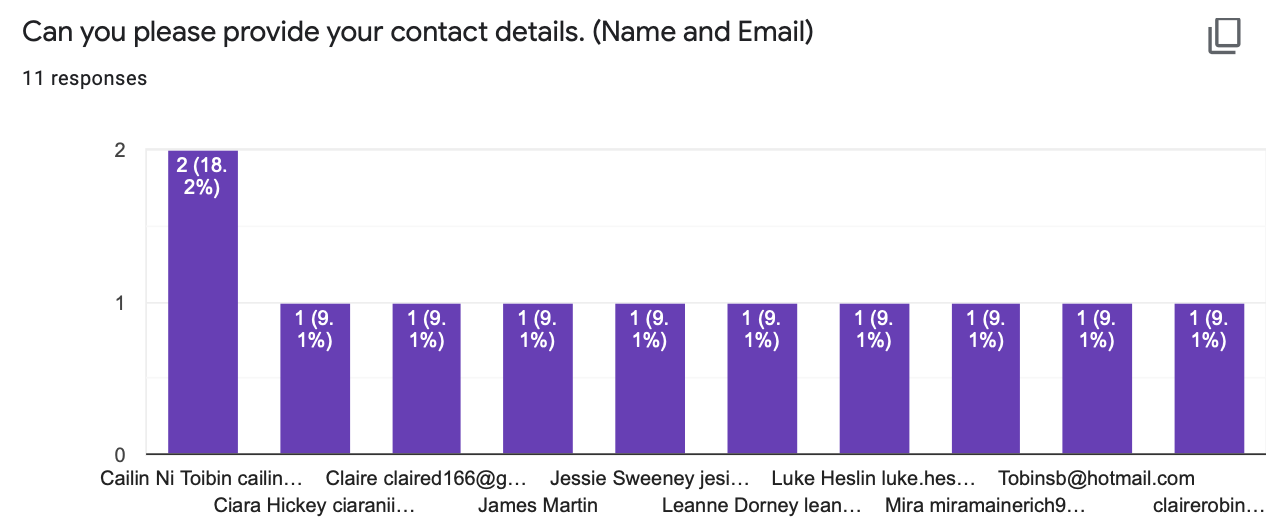
\includegraphics[width=1.0\textwidth]{IDD_LauraMartin_R00124705/Figures/respondentsSurvey2.png}
\caption{Details of participants}
{For question one, 11 respondents gave their name and email addresses.}
\end{figure}

\begin{figure}[b]
\centering
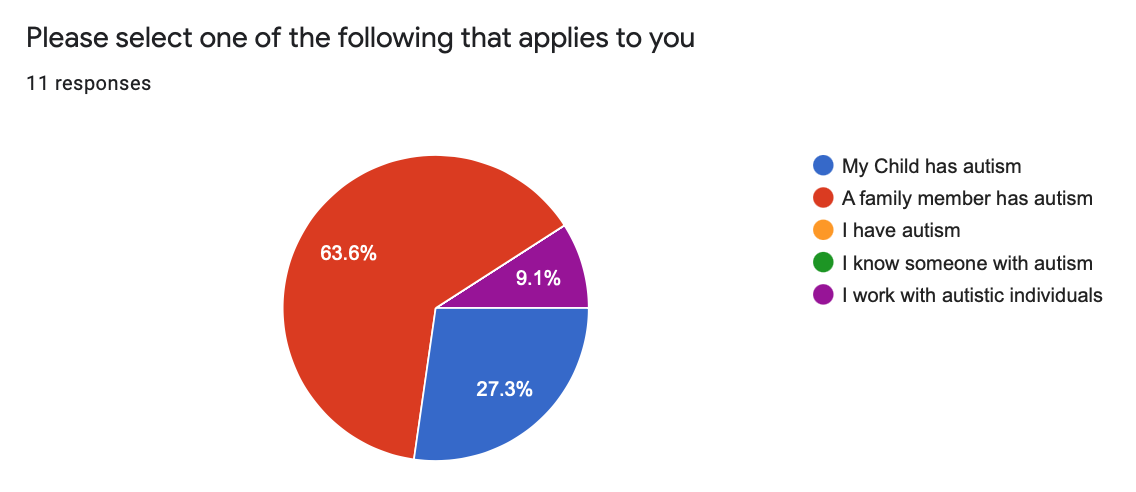
\includegraphics[width=1.0\textwidth]{IDD_LauraMartin_R00124705/Figures/survey1.png}
\caption{Relationship between respondent and person with Autism}
{For question two, 11 respondents answered their relationship to a person with Autism. The highest answer was the respondents have a family member with Autism, followed by their Child is Autistic and finally the respondents work with individuals who are Autistic}
\end{figure}


\begin{figure}[b]
\centering
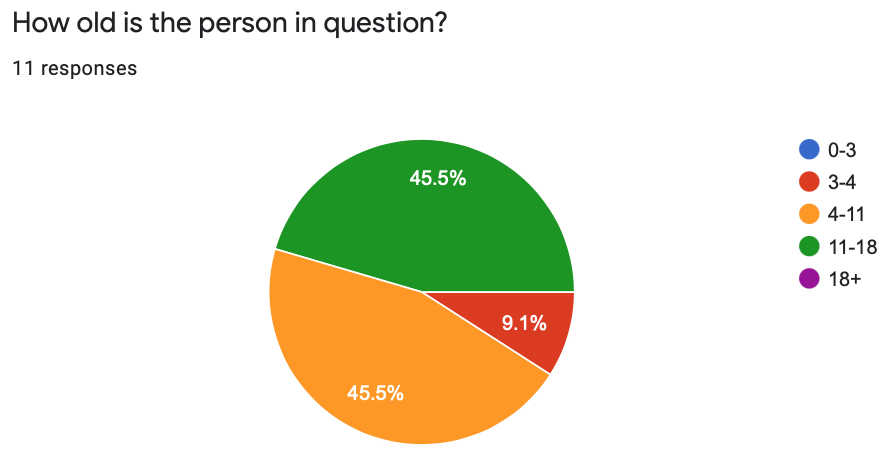
\includegraphics[width=1.0\textwidth]{IDD_LauraMartin_R00124705/Figures/survey2.png}
\caption{Pie chart representing the age of the individual with Autism.}
{For question three, 11 respondents answered a multiple choice question about their relationship to a person with Autism. The highest ages were those of school going ages. Ages between 11-18 was the most common, 4-11 was second and the least common was age 3-4 years old.}
\end{figure}


\begin{figure}[b]
\centering
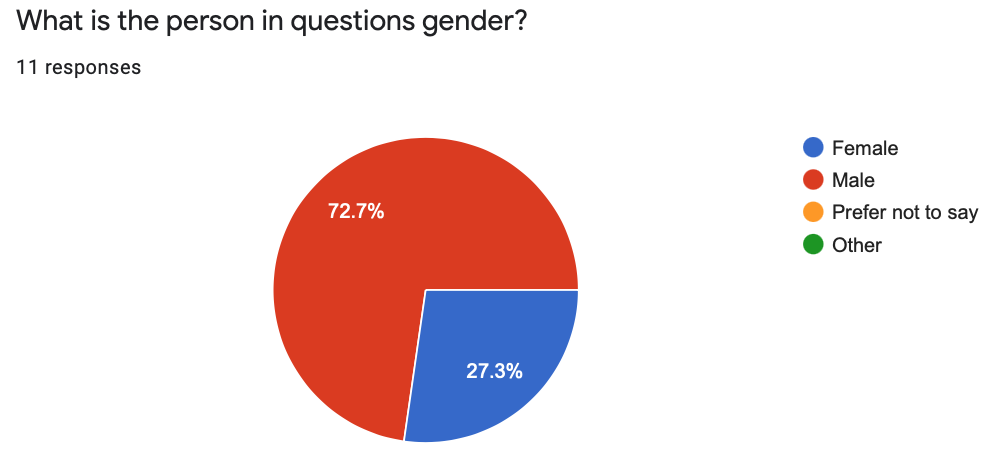
\includegraphics[width=1.0\textwidth]{IDD_LauraMartin_R00124705/Figures/survey3.png}
\caption{Pie chart representing the person in questions gender}
{For question four, 11 respondents answered a multiple choice question about the age of the person with Autism. The highest gender was Male at 72.7 percent and followed by female at 27.3 percent.}
\end{figure}

\begin{figure}[b]
\centering
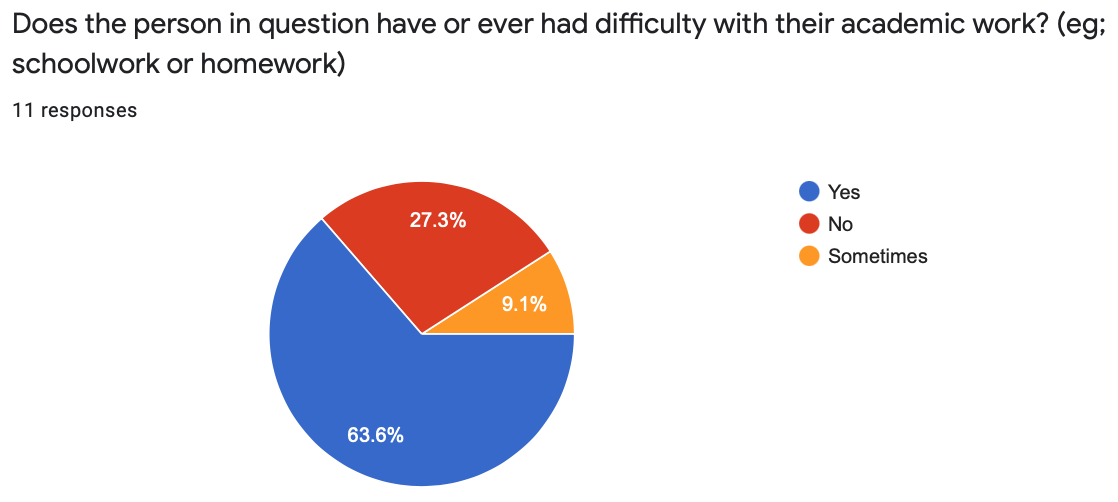
\includegraphics[width=1.0\textwidth]{IDD_LauraMartin_R00124705/Figures/survey4.png}
\caption{Pie chart representing the person in questions academic ability}
{For question five, 11 respondents answered a multiple choice question about the Autistic person in question and their ability in relation to their academic work.}
\end{figure}

\begin{figure}[b]
\centering
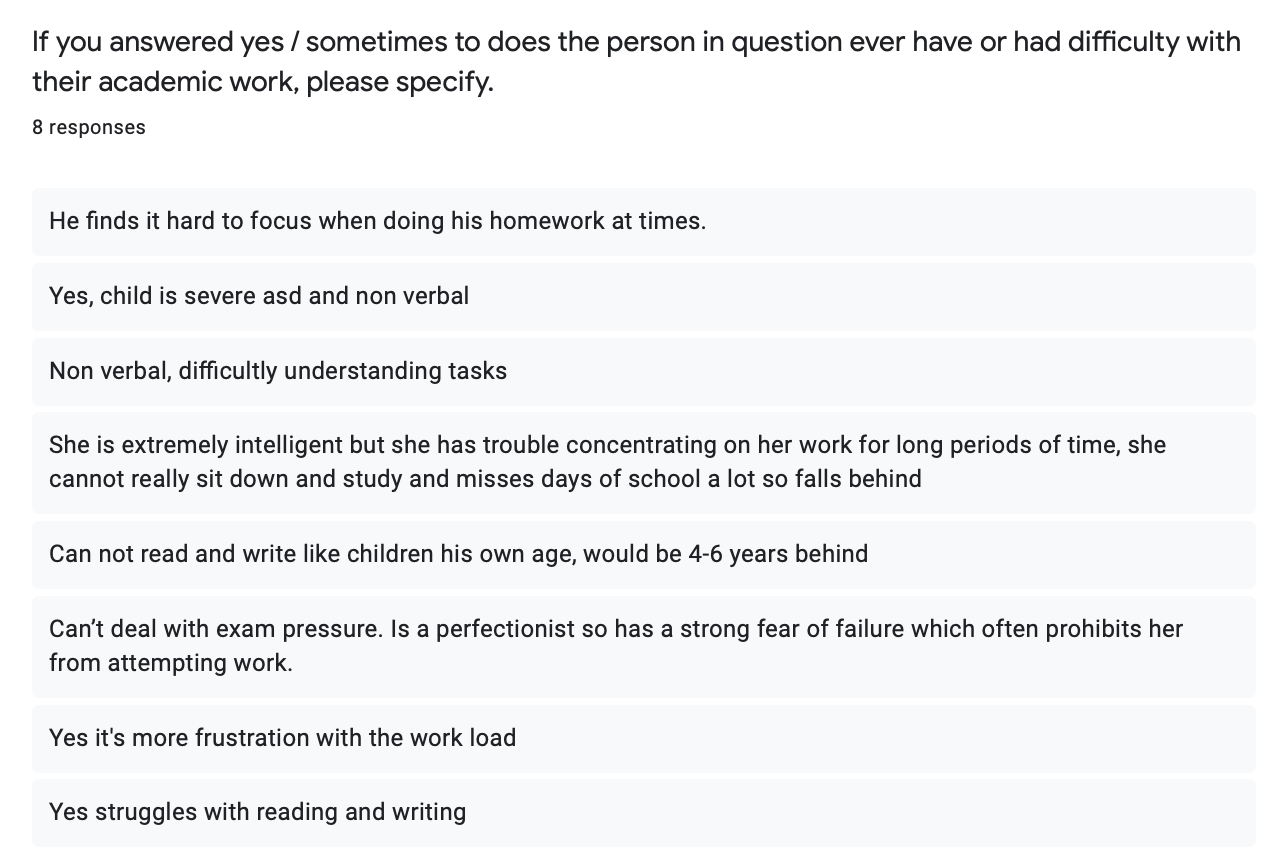
\includegraphics[width=1.0\textwidth]{IDD_LauraMartin_R00124705/Figures/academicdifficulty.png}
\caption{Academic difficulty answer box}
{For question six, 8 respondents were able to specify why the person with Autism does or sometimes struggles with their academic work.}
\end{figure}

\begin{figure}[b]
\centering
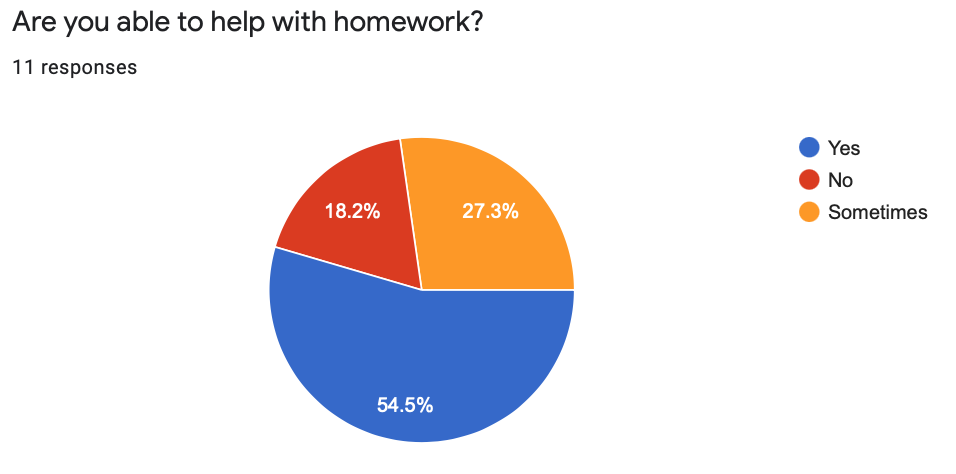
\includegraphics[width=1.0\textwidth]{IDD_LauraMartin_R00124705/Figures/survey5.png}
\caption{Does the respondent help with homework pie chart}
{For question seven, 11 respondents were given multiple choice questions about their ability to help the person in question with their homework.}
\end{figure}

\begin{figure}[b]
\centering
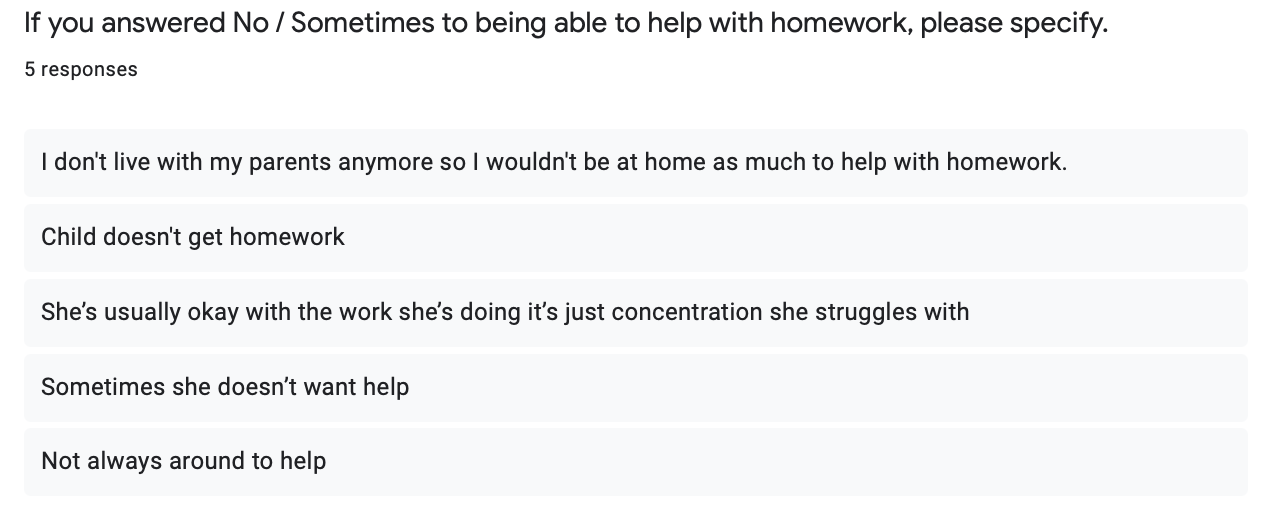
\includegraphics[width=1.0\textwidth]{IDD_LauraMartin_R00124705/Figures/homeworkhelp.png}
\caption{Helping with homework answer box}
{For question eight, 5 respondents gave their answer as to why they can not or only sometimes help the person with Autism and their homework. }
\end{figure}

\begin{figure}[b]
\centering
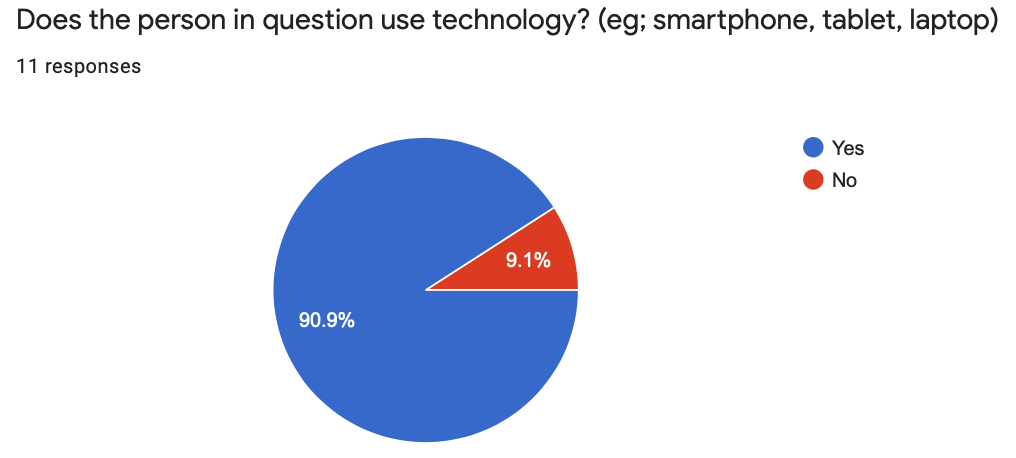
\includegraphics[width=1.0\textwidth]{IDD_LauraMartin_R00124705/Figures/survey6.png}
\caption{Does the person use technology}
{For question nine, 11 respondents answered does the person in question use technology.}
\end{figure}

\begin{figure}[b]
\centering
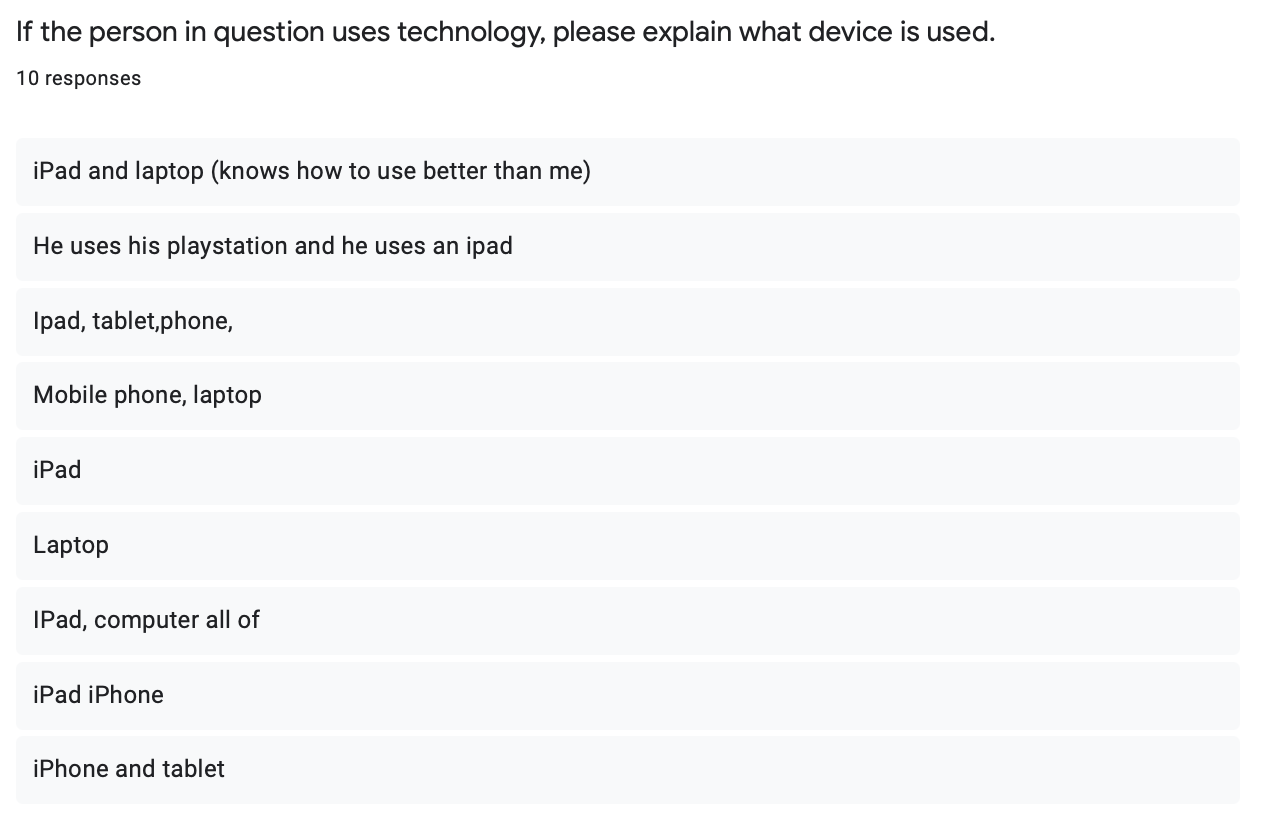
\includegraphics[width=1.0\textwidth]{IDD_LauraMartin_R00124705/Figures/technologyused.png}
\caption{What devices are used answer box}
{For question ten, 10 respondents answered what devices the person in question uses.}
\end{figure}

\begin{figure}[b]
\centering
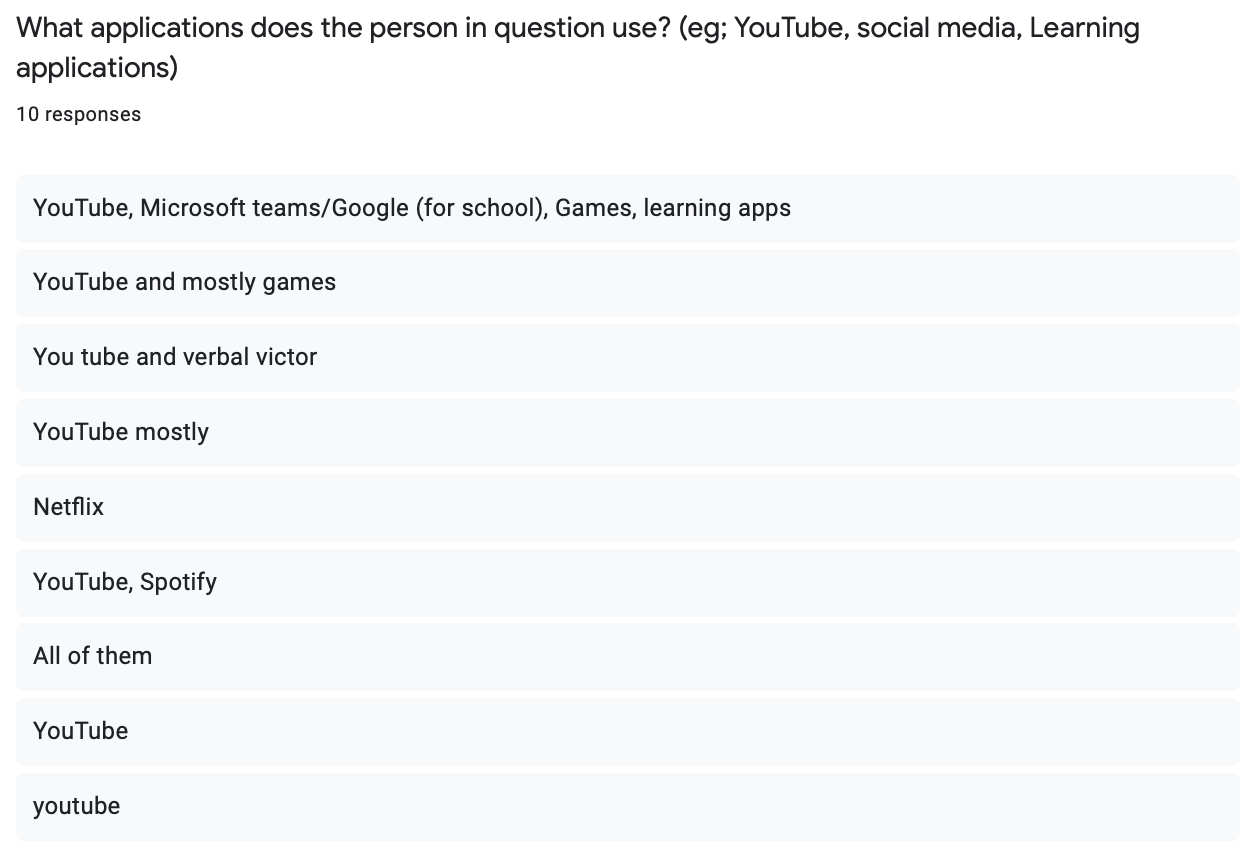
\includegraphics[width=1.0\textwidth]{IDD_LauraMartin_R00124705/Figures/applicationsused.png}
\caption{What applications are used answer box}
{For question eleven, 10 respondents answered what applications the person in question uses. }
\end{figure}

\begin{figure}[b]
\centering
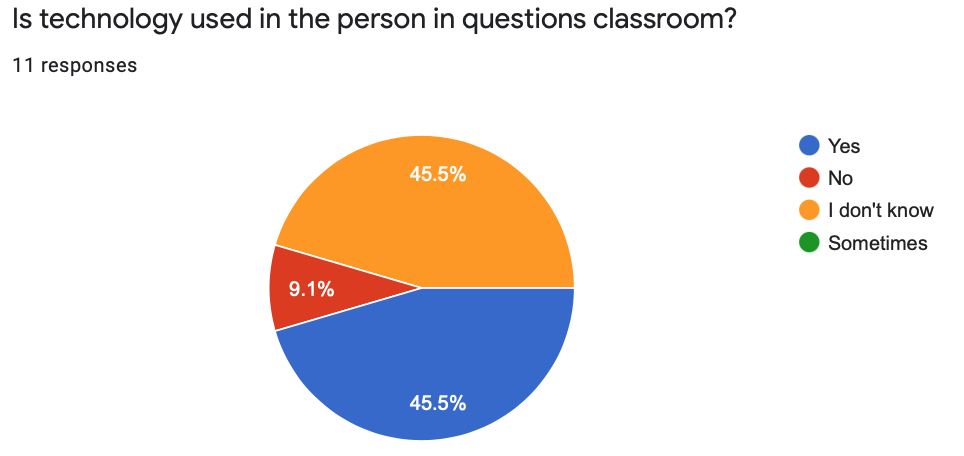
\includegraphics[width=1.0\textwidth]{IDD_LauraMartin_R00124705/Figures/survey7.png}
\caption{What devices are used pie chart}
{For question twelve, 11 respondents answered is technology used in the classroom of the individual with Autism. }
\end{figure}

\begin{figure}[b]
\centering
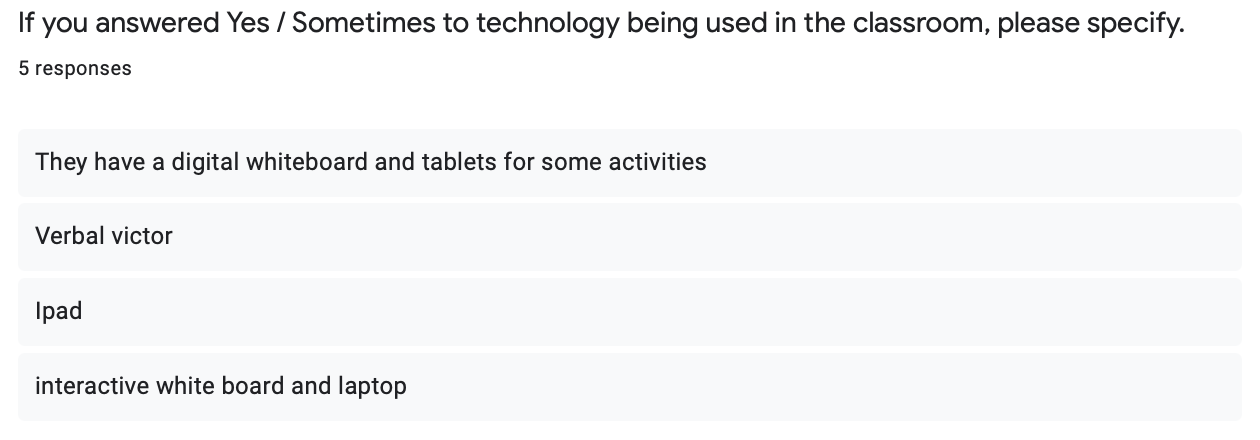
\includegraphics[width=1.0\textwidth]{IDD_LauraMartin_R00124705/Figures/classtechnology.png}
\caption{what technology is used answer box}
{For question thirteen, 5 respondents answered what technology devices are used in the classroom of the individual with Autism. }
\end{figure}

\begin{figure}[b]
\centering
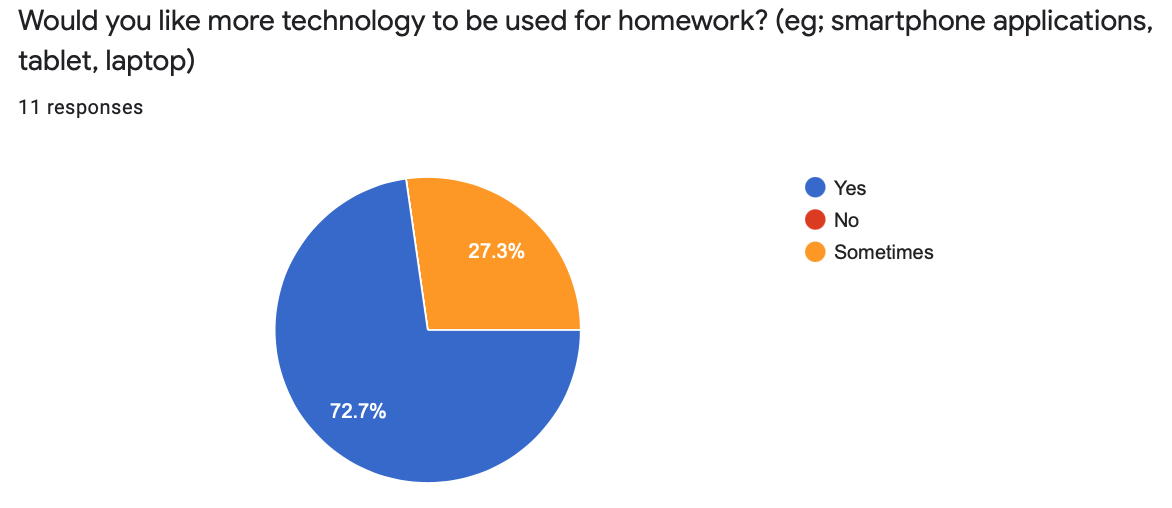
\includegraphics[width=1.0\textwidth]{IDD_LauraMartin_R00124705/Figures/survey8.png}
\caption{Technology devices pie chart}
{For question fourteen, 5 respondents answered what technology devices are used in the classroom of the individual with Autism. }
\end{figure}

\begin{figure}[b]
\centering
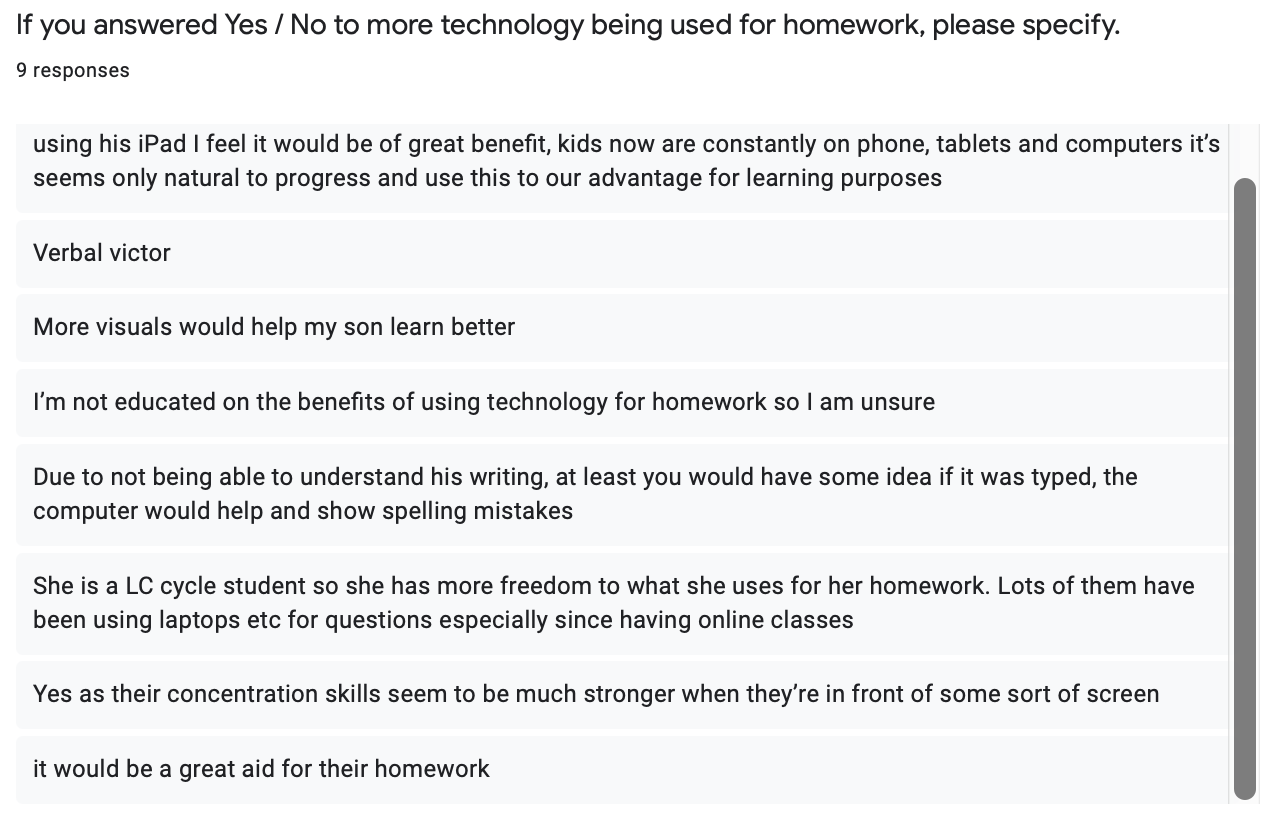
\includegraphics[width=1.0\textwidth]{IDD_LauraMartin_R00124705/Figures/moretechnologyused.png}
\caption{More technology answer box}
{For question fifteen, 9 respondents answered why more or less technology devices should be used for the person in question education. }
\end{figure}

\begin{figure}[b]
\centering
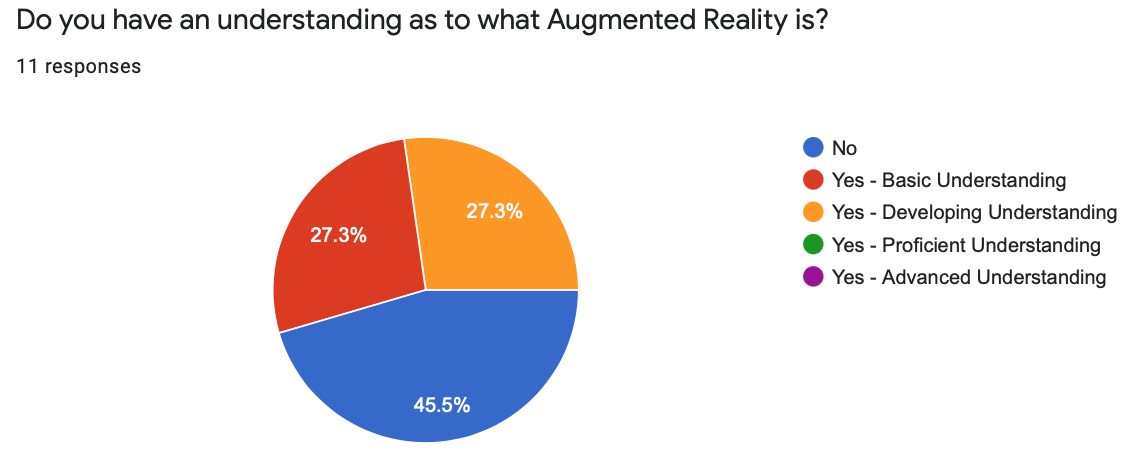
\includegraphics[width=1.0\textwidth]{IDD_LauraMartin_R00124705/Figures/survey9.png}
\caption{AR understanding Pie chart}
{For question sixteen, 11 respondents were given a multiple question about their understanding of AR.}
\end{figure}

\begin{figure}[b]
\centering
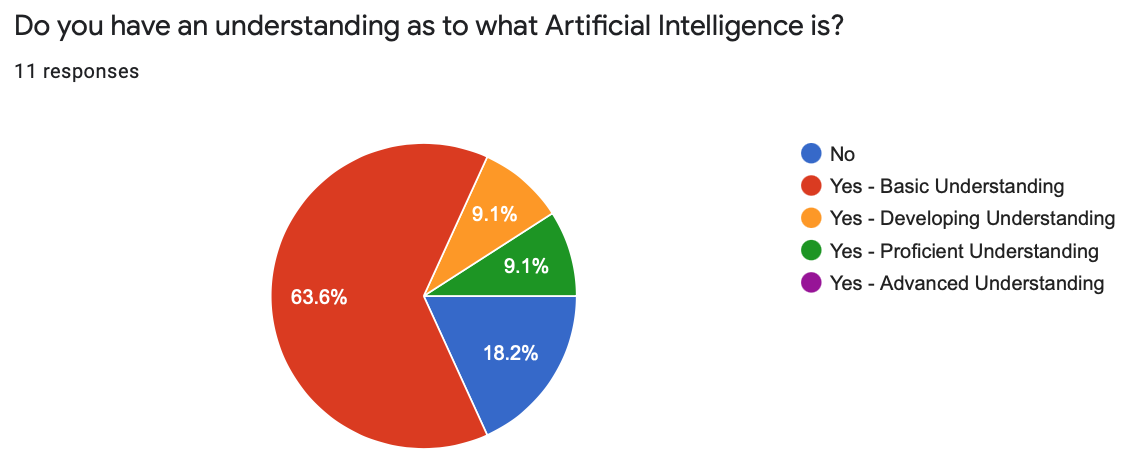
\includegraphics[width=1.0\textwidth]{IDD_LauraMartin_R00124705/Figures/survey10.png}
\caption{AI understanding Pie chart}
{For question seventeen, 11 respondents were given a multiple question about their understanding of AI.}
\end{figure}

\begin{figure}[b]
\centering
\includegraphics[width=1.0\textwidth]{IDD_LauraMartin_R00124705/Figures/furtherhelp.png}
\caption{Further information answer box}
{For question seventeen, 7 respondents gave their feedback of information that may further help my study.}
\end{figure}

\subsection{Survey two analysis}

\begin{table} [b]
    \centering
\begin{tabular}{ | m{3em} | m{10cm}| } 
\hline
Q1. & There is a good range of occupations that are related to the target audience. \\ 
\hline
Q.2 & This question gave the details of the participants, it concluded of their name and email address for further contact. \\ 
\hline
Q.3 & 100 percent of the participants educates a person with Autism, this is crucial for feedback and design going foreword.  \\ 
\hline
Q.4 & 83.3 percent of the respondents educated children with Autism who were the school going age of 4-11, this is vital information as that is the age of the demographic for the proposed application.  \\ 
\hline
Q.5 & 83.3 percent of the respondents educated children in a mixed gender school, while 16.7 percent taught in a all male school. This is interesting feedback as none of the applicants educated in an all female school.  \\ 
\hline
Q.6 & 83.3 percent of the respondents claimed their students struggled with either their homework or their school work and 16.7 percent had some difficulty. This result was to be expected as the Children are learning new skills and having a learning disability typically can make this challenging.   \\ 
\hline
Q.7 & 87.5 percent of the participants use technology in the class while 12.5 percent only sometimes use technology, this can be put down to limitations, resources and internet connection in the school. \\ 
\hline
Q.8 & All respondents explained what devices they used in the classroom, the most common answer was a form of tablet and an interactive whiteboard. \\ 
\hline
Q.9 & 100 percent of the respondents used a form of technology for educating students with Autism. \\ 
\hline
Q.10 & The respondents explained what form of devices they used to educate a student with Autism, the most common answer was an interactive whiteboard and a form of table. \\ 
\hline
Q.11 & 100 percent of the respondents used a child centered approach when educating students with Autism, this is expected as it is a recommend form of practice for individuals with Autism as ability can vary. \\ 
\hline
Q.12 & 75 percent of respondents used the internet as part of their studies, while 25 percent did not. This is interesting as due to the COVID-19 pandemic all schools in Ireland for a period of time had to migrate to teaching online. \\ 
\hline

Q.13 & Respondents gave an explanation as to why students would access the internet as part of their studies, the main reasons were accessing information for a project, or using the internet to access the curriculum or SeeSaw, an online learning portal for schools.  \\
\hline
Q.14 & 50 percent of respondents used a camera as part of their studies, while 50 percent did not. This was interesting as half the respondents did not use a camera to track students progress while education was online.  \\
\hline
Q.15 & 50 percent of respondents used a smart device camera as part of their studies, while 50 percent did not. This is not surprising as the same results appeared in question 14.  \\
\hline
\end{tabular}
\centering

\caption{Survey two analysis}
    \label{tab:my_label}
\end{table}




 % Discussion and Conclusion
\chapter{Implementation of design}
\label{chap:Prototype Design}
\lhead{\emph{Implementation of design}}





 % Discussion and Conclusion
\chapter{Prototype Design}
\label{chap:Prototype Design}
\lhead{\emph{Prototype Design}}

\section{Proposed Prototypes}

here goes influence of design, reasoning of design, feedback from survey for design,
put images side by side and more prototypes


\begin{figure}[h]
\centering
\includegraphics[width=0.5\textwidth]{IDD_LauraMartin_R00124705/Figures/prototype-01.jpg}
\caption{Prototype one}
{For question seventeen, 7 respondents gave their feedback of information that may further help my study.}
\end{figure}

\begin{figure}[h]
\centering
\includegraphics[width=0.5\textwidth]{IDD_LauraMartin_R00124705/Figures/prototype-02.jpg}
\caption{Prototype two}
{For question seventeen, 7 respondents gave their feedback of information that may further help my study.}
\end{figure}

\begin{figure}[h]
\centering
\includegraphics[width=0.5\textwidth]{IDD_LauraMartin_R00124705/Figures/prototype-03.jpg}
\caption{Prototype three}
{For question seventeen, 7 respondents gave their feedback of information that may further help my study.}
\end{figure}

\begin{figure}[h]
\centering
\includegraphics[width=0.5\textwidth]{IDD_LauraMartin_R00124705/Figures/prototype-04.jpg}
\caption{Prototype four}
{For question seventeen, 7 respondents gave their feedback of information that may further help my study.}
\end{figure}

\subsection{Analysis of prototype}
This is my problem, this sub section is meant to be on page after pg 54




%\documentclass[10pt,a4paper]{article}
%\usepackage[demo]{graphicx}
%\usepackage{subfig}
%\begin{document}
%\begin{figure}
    %\centering
    %\includegraphics[width=0.5\textwidth]{IDD_LauraMartin_R00124705/Figures/prototype-01.jpg}
    %\qquad
    %\subfloat[label 2]{{\includegraphics[width=5cm]{img2} }}
    %\caption{2 Figures side by side}
    %\label{fig:example}
%\end{figure}
%\end{document} % prototype


%% ----------------------------------------------------------------
\label{Bibliography}
\bibliographystyle{IEEEtranN}  % Use the "IEEE Transaction" BibTeX style for formatting the Bibliography
\bibliography{Information/Bibliography}  % The references (bibliography) information are stored in the file named "Bibliography.bib"
\lhead{\emph{Bibliography}}  % Change the left side page header to "Bibliography"

%% ----------------------------------------------------------------
% Now begin the Appendices, including them as separate files

\addtocontents{toc}{\vspace{2em}} % Add a gap in the Contents, for aesthetics

\appendix % Cue to tell LaTeX that the following 'chapters' are Appendices

\chapter{Code Snippets}

Put appendix material in this section e.g. code snippets 

 If there is too much code to include in the Appendix, submit the rest on a USB disk or CD. Some code should be easily available for examiners to assess.
 
USE THE APPENDICES	% Appendix A
\chapter{Wireframe Models} % Appendix B


\addtocontents{toc}{\vspace{2em}}  % Add a gap in the Contents, for aesthetics
\backmatter
\end{document}  % The End
%% ----------------------------------------------------------------